\documentclass{acm_proc_article-sp}

\usepackage{color}
\usepackage{graphicx}
\newcommand{\TODO}[1]{\textcolor{red}{{\bf TODO:} #1}}
\newcommand{\checkme}[1]{\textcolor{red}{\textbf{#1}}}



\usepackage{etoolbox}
\makeatletter
\patchcmd{\maketitle}{\@copyrightspace}{}{}{}
\makeatother

\begin{document}

\title{Flat Combining Synchronized Global Data Structures}
\titlerunning{Flat Combining Synchronized Global Data Structures}

% from the submissions guidelines: On the front page, in place of the authors'
% names, the paper should indicate: the paper ID number assigned during the
% paper registration process and the total number of pages in the submission.a

\author{
Brandon Holt\inst{1}
\and Jacob Nelson\inst{1}
\and Brandon Myers\inst{1}
\and Preston Briggs\inst{1}
\and Luis Ceze\inst{1}
\and Simon Kahan\inst{1,2}
\and Mark Oskin\inst{1}
}

\institute{
  University of Washington
\and
  Pacific Northwest National Laboratory\\
  \email{\{bholt,nelson,bdmyers,preston,luisceze,skahan,oskin\}@cs.washington.edu}
}

\authorrunning{Holt, Nelson, Myers, Briggs, Ceze, Kahan, Oskin}

% \author{Brandon Holt}
% \authorinfo{Brandon Holt$^{\dagger}$,
%   Jacob Nelson$^{\dagger}$,
%   Brandon Myers$^{\dagger}$,\\
%   Preston Briggs$^{\dagger}$,
%   Luis Ceze$^{\dagger}$,
%   Simon Kahan$^{{\dagger \ddagger}}$,
%   Mark Oskin$^{\dagger}$
% }{\textdagger University of Washington, \textdaggerdbl Pacific Northwest National Laboratory}{
%   \{bholt, nelson, bdmyers, preston, luisceze, skahan, oskin\}@cs.washington.edu}
% 
% \toappearbox{To appear in PGAS'13}

\clearpage

\maketitle
\begin{abstract}
\Grappa is a runtime system for commodity clusters of multicore computers that
presents a massively parallel, single address space abstraction to
applications. \Grappa's purpose is scalable performance for irregular
parallel applications, such as graph processing. Poor data locality, imbalanced parallel
work and complex communication patterns make these applications difficult to scale.

\Grappa serves both as a C++ user library and as a foundation upon which
higher level languages can be developed or adapted. \Grappa tolerates delays
to remote memory by multiplexing thousands of lightweight workers
to each processor core; balances load via fine-grained distributed
work-stealing; increases communication throughput by aggregating
smaller data requests into large ones; and provides efficient synchronization
and remote operations. We present a detailed description of the \Grappa
system and
%programming examples using the library interface,
performance comparisons on several irregular benchmarks to hand-optimized MPI code and to
the Cray XMT, a custom system used to target the real time graph analytics
market.

\end{abstract}

\TODO{Refine/fix discussion of ``linearizability'' and ``serializability'' to use terminology precisely.}

\section{Introduction}
% - PGAS languages successfully bring shared memory problems into distributed memory systems
% - Cost functions are different, but many of the other considerations, such as reducing locking, still apply
% - With abundant parallelism, we can tolerate some serialization to reduce number of synchronizations and reduce overall communication

The goal of partitioned global address space (PGAS) languages and runtimes is to provide the illusion of a single shared memory to a program that actually executes on a number of machines each with their own memory. This allows programmers to write their algorithms without needing to explicitly manage communication. Once the algorithm is correct, many techniques exist to help improve performance improving locality (spatial and temporal) and coarsening communication where possible. However, with this shared memory abstraction come all of the difficult concurrency issues that arise in physically-shared memory. Luckily, there exists a large body of work solving these issues in physically-shared memory which the PGAS community can leverage. The opportunity here is that, in a distributed setting, the costs of communication and synchronization operations are different, so different performance trade-offs will be made.

Globally-shared data structures are one of the cornerstones of shared-memory and PGAS abstractions. 
In order for multiple concurrent threads to interact with one another, they must observe shared data consistently. It is commonly accepted that the easiest consistency model to reason about enforces that all accesses appear to happen in some serializable order that all threads agree on (known as \emph{sequential consistency or SC}).
However, in both physically-shared memory and PGAS, maintaining this sequentially consistent view of data among all concurrently accessing threads presents performance challenges.
The simplest way to maintain SC for a given data structure is to have a single global lock that implements mutual exclusion and enforces a serializable order over read and write operations. The cost of literally serializing accesses in this way is typically considered prohibitive, even in physically shared memory.
With the massive amount of parallelism in a cluster of multiprocessors and with the increased cost of remote synchronization, the problem magnifies.

Prior work on shared memory has explored the scalability challenges of adding more concurrent accessors to shared data structures.
% One observation was that, when multiple threads of control concurrently access the same object, they can conduct themselves in one of two ways: contend or cooperate.
In the classic case of contention, either all threads fight to obtain a single global lock, or they attempt a series of potentially-contended atomic operations in the case of a more advanced synchronization strategy such as a lock-free queue. In both cases, as the number of concurrent accessors increases, the more they contend and the more failed synchronization operations there are.
The observation of previous work was that the cost of many of these failed synchronization attempts can be mitigated by having the threads \emph{cooperate} via delegation rather than \emph{contend}.
If multiple threads delegate a single thread to do all of their operations, they can avoid excessive synchronization overhead on ``hot'' locations.

The trick is coming up with a mechanism for delegating that has lower synchronization overhead than the original contention case.
Prior work showed that a cleverly-implemented ``publication list'' can allow multiple accessors to cooperate with minimal synchronization.
This same work makes the additional observation that, given the semantics of some particular data structures, the set of accesses being serialized can be composed and performed more efficiently \emph{combined} than individually, which they dub \emph{flat combining}.
Together, the reduced synchronization cost and combined operations allow even a data structure with a single global lock to scale better than complicated concurrent data structure implementations with fine-grained locking.
Further, the same publication list mechanism can be applied to other data structures, and all that must be customized is the particular way in which operations for a given data structure can be combined.

% Make this point later?
% In many cases, algorithms do not require operations to be immediately consistent. Many optimizations for message-passing or PGAS-style distributed memory algorithms leverage this observation to minimize the need for fine-grained communication. However, they typically must make this visible to programmers, who now must take care to insert their own memory barriers where appropriate, or otherwise express the way in which consistency relaxation can occur.

The goal of this work is to apply the concept of flat-combining in a PGAS runtime to reduce the cost of maintaining globally consistent data structures in a generic way.
To evaluate this, we leverage the Grappa runtime~\cite{Nelson:hotpar11-real}, a PGAS-style runtime library optimized for fine-grained random access, which provides the ability to tolerate long latencies by efficiently switching between many lightweight threads.
With enough concurrent threads, it is actually possible to maintain program order within each thread by blocking on accesses, but still have an opportunity to effectively combine many fine-grained synchronous operations for better performance.
With the same flat-combining mechanism, multiple global data structures can be implemented efficiently, even with simple locking schemes.

% lay out the upcoming sections of the paper...
The next section will describe in more detail the Grappa runtime system that is used to implement flat combining for distributed memory machines. Then we explain the flat combining mechanism in more depth and describe how it maps to a PGAS model. Next we explain how several data structures are implemented in this framework and show how they perform on simple throughput workloads. Finally, we evaluate how they affect performance when used in a simple application kernels.

\section{Grappa} \label{sec:grappa}

\begin{figure}[t]
\begin{center}
  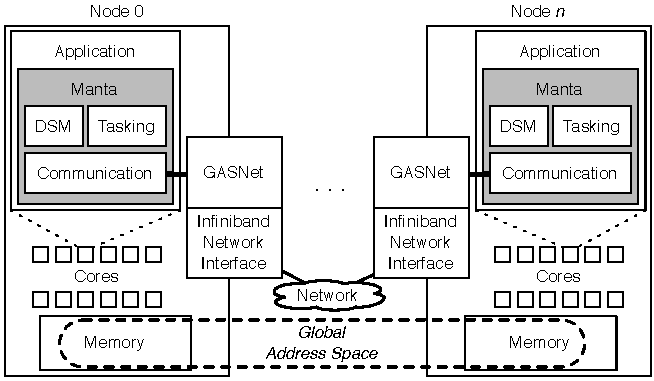
\includegraphics[width=0.95\columnwidth]{figs/system-overview}
\begin{minipage}{0.95\columnwidth}
  \caption{\label{fig:grappa} Grappa system overview}
\end{minipage}
\vspace{-3ex}
\end{center}
\end{figure}

The Grappa runtime system (Figure~\ref{fig:grappa}) supports scaling of irregular applications via three key components:
a \textbf{distributed shared global memory} providing high aggregate random access bandwidth for both normal and synchronized operations;  
a \textbf{tasking system} with lightweight multithreading to tolerate latency and workstealing to automate load balance;
and a \textbf{communication layer} using network packet scheduling and aggregation to achieve high performance while remaining largely invisible to applications.
Unlike many runtime systems where the task scheduler, memory access manager, and the communication  are separable subsystems, in Grappa these three components are tightly integrated and the performance of each depends heavily on that of the other two.  For example, eficiency of the communication layer requires that the tasking system multiplex tasks -- and the memory manager fetch data -- sufficiently rapidly to aggregate hundreds of individual requests into each packet; otherwise, the network will be poorly utilized.  Nonetheless, for simplicity of exposition, we describe each component in turn.

We now discuss the
programmer's view of Grappa's main capabilities, including a subset of
the Grappa API. In Section~\ref{implementation}, we discuss the details
of their implementation.

\TODO{Should we have a code example here, and walk thru it as we explain the
components and parts of the API?}

\subsection{Tasks}

%The basic unit of locality in Grappa is the {\em core}. Each core is
%responsible for a section of the global memory

The basic unit of execution in Grappa is a {\em task}. Tasks are
small; just a function pointer and arguments. Tasks are only
queued when they are spawned; later, when resources are free, they are
allocated a stack, bound to a core, and executed.

Grappa's tasks give up control of their core when when they perform
long-latency operations, allowing the processor to remain busy while
waiting for the operation to complete. This is most often done
implicitly inside a call into Grappa's API, but it can also be done
explicitly by the programmer using the calls shown in
Figure~\ref{fig:scheduling}. \TODO{cite UPC split phase reads and
writes, but include that we provide a way to overlap computation}

All Grappa scheduling is done in userspace, and minimal state is saved,
in order to minimize the context switch time. In our experiments, we saw
context switch times as low as \checkme{40ns}. This lightweight context
switching is Grappa's key enabling feature. It gives us the ability to
tolerate latency. Given that ability, we are able to \textbf{trade
latency for throughput}: by {\em increasing} latency in key components
in the system we are able to increase our aggregate random access
bandwidth, our synchronization bandwidth, and our ability to tolerate
load.

\begin{figure}[htbp]
  \begin{center}
    \begin{description}\small
    \item[ \texttt{ yield() } ] \hfill \\
      Gives up control of core to scheduler, queuing task to be scheduled again soon
    \item[ \texttt{ suspend() } ] \hfill \\
      Gives up control of core to scheduler
    \item[ \texttt{ wake( task * $t$ ) } ] \hfill \\
      Enqueues $t$ to be scheduled again soon
    \end{description}
    \begin{minipage}{0.95\columnwidth}
      \caption{\label{fig:scheduling} Grappa API: scheduling} %{-4ex}}
    \end{minipage}
    %\vspace{-3ex}
  \end{center}
\end{figure}


\subsection{Expressing parallelism}

A programmer's goal in coding with Grappa should be to express as much
parallelism as possible without worrying about where it will execute.
Grappa then chooses where and when to exploit this parallelism,
scheduling as much work as necessary to tolerate network latencies and
keep cores busy. 

Grappa provides four methods for expressing parallelism, shown in
Figure~\ref{fig:expressing-parallelism}. The first is explicit task
spawns. When the programmer identifies work that can be done in
parallel, the work may be wrapped up in a function and queued with its
arguments for later execution using a \texttt{spawn}. If the
programmer wishes to spawn a task on a specific core in the system,
or at the home core of a particular memory location, Grappa provides a
\texttt{spawn\_on} call for this purpose.

The next method for expressing parallelism is a parallel for loop, where
the number of iterations must be known at loop entry. The programmer
specifies a function pointer along with start and end indices and an
optional threshold to control parallel overhead. Grappa does {\em
recursive decomposition} of iterations, similar to Cilk's cilk\_for
construct~\cite {cilkforimplementation} \comment{could only find slides
page6 of
http://www.clear.rice.edu/comp422/lecture-notes/comp422-2012-Lecture5-
Cilk++.pdf    ---- Good enough.  Cite it.  -Mark}.  It generates a
logarithmically-deep tree of tasks, stopping to execute the loop body
when the number of iterations is below the required threshold. Finally,
a programmer may want to run a small piece of code on a particular core
in the system without waiting for execution resources to be available.
Grappa provides the \texttt{call\_on} call for this purpose.

\begin{figure}[htbp]
  \begin{center}
    \begin{description}\small
    \item[ \texttt{spawn( void (*fp)(args) )} ] \hfill \\
      Creates a new stealable task
    \item[ \texttt{spawn\_on( core, (*fp)(args) )} ] \hfill \\
      Creates a new private task that will run on a specific core 
    \item[ \texttt{parallel\_for( (*fp)(args), start, end )} ] \hfill \\
      Executes iterations of a loop as stealable tasks 
    \item[ \texttt{call\_on( core, (*fp)(args) )} ] \hfill \\ 
      Runs a limited function on a specific core without consuming
      Grappa execution resources 
    \end{description}
    \begin{minipage}{0.95\columnwidth}
      \caption{\label{fig:expressing-parallelism} Grappa API: expressing parallelism} % \vspace{-4ex}}
    \end{minipage}
    %\vspace{-3ex}
  \end{center}
\end{figure}

\subsection{Memory}

Applications written for Grappa utilize two forms of memory: local and
global.

Local memory is local to a single core in the system.  Accesses occur
through conventional pointers.  The compiler emits an access and the
memory is manipulated directly.  Applications use local accesses for a
number of things in Grappa: the stack associated with a task, accesses
to localized global memory in caches (see below), and accesses to
debugging infrastructure that is local to each system node.  Local
pointers cannot access memory on other cores, and are valid only on
their home core.

Large data that is expected to be shared and accessed with low locality is
stored in Grappa's global memory. All global data must be accessed through
calls into Grappa's API, shown in Figure~\ref{fig:accessing-memory}.

\paragraph{Global memory allocation}
Grappa provides two methods for {\emph storing} data in the global memory. The
first is a distributed heap striped across all the machines in the
system. The \texttt{global\_malloc} and \texttt{global\_free} calls
are used to allocate and deallocate memory in the global heap; on
allocation, a global pointer is returned. Grappa also allows any local
data on a core's stacks or heap to be exported to the global address
space to be made accessible to other cores across the system.

\paragraph{Global memory access} There are two approaches to {\emph
accessing} global memory. When the programmer expects a computation on
shared data to have spatial locality to exploit, {\em cache} operations
may be used. When there is no locality to exploit, {\em delegate}
operations are used. Since these operations are expected to communicate
with other nodes and have high latency, cache and delegate operations
interact with the scheduler; when issuing a long-latency request, they
suspend the requesting task and allow the core to execute other work
until their response arrives.

\paragraph{Explicit caching} With Grappa's explicit caching support,
applications can instruct Grappa to fetch a global pointer of any length
and return a local pointer to a cached copy of the global memory. Under
the hood, Grappa performs the mechanics of gathering chunks of data from
multiple system nodes and presenting a conventional appearing linear
block of memory as a pointer into a cache. Grappa cache operations have
the usual read-only and read-write variants, along with a write-only
variant used to initialize data structures. Cache operations exploit
spatial locality by reducing the number of small network messages
accessing contiguous data. Languages for distributed shared memory
systems have done optimizations to achieve a similar goal. For example,
the UPC compiler coalesces struct and array accesses into remote get/put
\cite{Chen:2005}, and Fortran D compiler's message vectorization hoists
small messages out of a loop \cite{FortranD:1992}. Caching in Grappa
additionally provides a mechanism for exploiting temporal locality by
operating on the data locally. 

\paragraph{Delegate operations}
When the access pattern has low-locality, it is more efficient
to modify the data on its home core rather than bringing a copy to the
requesting core and returning it after modification. Delegate
operations provide this capability. Applications can dispatch
computation to be performed on individual machine-word sized chunks of
global memory to the memory system itself (e.g.,
\emph{fetch-and-add}). \comment{should we bring up delegation in the intro?}

Delegate operations, proposed in \cite{Nelson:hotpar11}, are also the
primary synchronization method in Grappa. Each piece of global memory is
paired with a single core in the system; all accesses to that actual
memory location are done by that core. This allows delegate operations
to be performed atomically on the core simply by making sure no other
code interleaves their operation; and, since context switches in Grappa
are cooperative, this is trivial. Thus, delegate operations are able to
provide atomic semantics to memory owned by one core without using
atomic operations. Using delegation to implement isolation for any
subset of memory has been explored in \cite{delegated:oopsla11}.

\begin{figure}[htbp]
  \begin{center}
    \begin{description}\small
      \item[ \texttt{ global\_address global\_malloc( size )} ] \hfill \\
      \item[ \texttt{ global\_free( global\_address )} ] \hfill \\
        Allocates and frees memory in the global heap
      \item[ \texttt{ delegate\_read( global\_address, local\_var )} ] 
      \item[ \texttt{ delegate\_write( global\_address, local\_var )} ] %\vspace{-2ex}
      \item[ \texttt{ delegate\_cas( global\_address, local\_var )} ] %\vspace{-2ex}
      \item[ \texttt{ delegate\_inc( global\_address, local\_var )} ] %\vspace{-2ex} 
\hfill \\
        Performs a memory operation at the home core of a global address
      \item[ \texttt{ cache\_acquire( global\_address, local\_buf, \{RO,RW,WO\})} ]
      \item[ \texttt{ cache\_release( global\_address, local\_buf )} ] %\vspace{-2ex} 
\hfill \\
        Perform cache operations \TODO{expand}
    \end{description}
    \begin{minipage}{0.95\columnwidth}
      \caption{\label{fig:accessing-memory} Grappa API: accessing memory} %{-4ex}}
    \end{minipage}
    %\vspace{-3ex}
  \end{center}
\end{figure}


\section{Flat Combining}

At the most basic level, the concept of flat combining is about enabling cooperation among threads rather than contention. The benefits can be broken down into three components: improved locality, reduced synchronization, and data structure-specific optimization. We will explore how this works in a traditional shared memory system, and then describe how the same concepts can be applied to distributed memory.

% Flat combining allows threads to cooperate when accessing a synchronized shared data structure to get greater overall throughput than even each of them operating serially. However, the same delegation mechanism can be reused in any data structure protected by a single global lock. 

\subsection{Physically-shared memory}

\begin{figure}[ht]
  \centering
  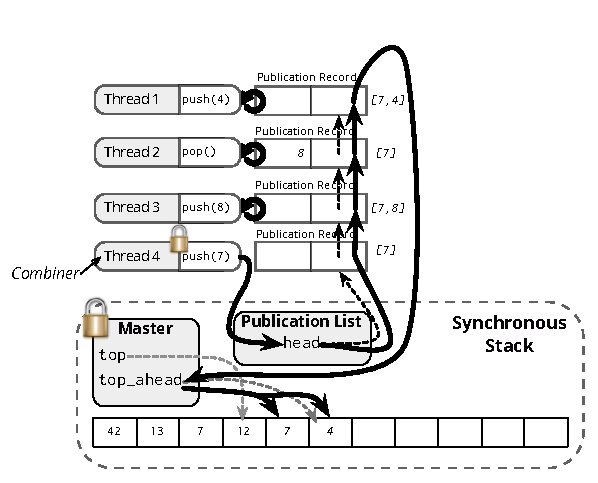
\includegraphics[width=0.5\textwidth]{figs/fc_shared_mem.pdf}
  \caption{\emph{Flat combining in shared memory.}
    To access the shared stack, each thread adds its request to the publication list (1). Thread 4 acquires the stack's lock and becomes the combiner (2), while the remaining threads spin waiting for their request to be satisfied. The combiner walks the publication list from the head, matching up Thread 3's push with Thread 2's pop on its own private stack (3). The 2 remaining pushes are added to the top of the shared stack (4). Finally, the top is updated, and Thread 4 releases the lock and continues its normal execution.
  }
  \label{fig:fc_shared_mem}
\end{figure}

One of the issues with shared data structures in a shared-memory multicore is that threads executing on different cores will force the hottest parts of the data structure to thrash between their caches. Having a single thread do all of the operations on the data structure allows it to keep everything in its cache.

% Improving locality in a shared-memory multicore is achieved by 
% Having a single thread bound to a particular core do a string of accesses trivially results in a lower cache miss rate than having multiple threads on multiple cores bring the data structure into cache each in turn.

% Careful engineering must be employed to implement a mechanism for cooperation that does not introduce the same synchronization issues as the original contended data structure.

Reduced synchronization comes from delegating work to another core.
To illustrate the issue, consider the shared synchronous queue, shown in Figure~\ref{fig:fc_shared_mem}, with pre-allocated storage and a \texttt{top} pointer protected by a lock. Without flat combining, whenever a thread attempts to push something on the stack, it must acquire the lock, put its value into the storage array, bump the top, and then release the lock. When many threads contend for the lock, all but one will fail and will have to retry. Each try forces a memory fence for consistency and consumes bandwidth, and as the number of threads increases, the fraction of successes plummets. Under flat combining, instead, threads add requests to the publication list. They each try to acquire the lock, and the one that succeeds becomes the combiner. Instead of retrying, the rest spin waiting for their request to be filled. The combiner walks the publication list, performs all of the requests, and when done, releases the lock. This has greatly reduced the synchronization on the stack's lock, but has introduced a new point of synchronization---threads must synchronize to add to the publication list. However, if a thread performs multiple operations on the stack, it can leave its publication record in the list and amortize the synchronization cost.

The above example of delegation is compelling in itself. However, the crux of the prior work is that data structure-specific optimization can be done to perform the combined operations more efficiently than separately.
As the combiner walks the publication list, it merges each non-empty publication record into a combined operation. In the case of the stack example shown in Figure~\ref{fig:fc_shared_mem}, as it walks the list, Thread 4 keeps track of the operations on its own temporary stack. When it encounters Thread 2's pop, it recognizes that it can satisfy that pop immediately with the push it just processed from Thread 3, so it fills each of their records and allows each of them to proceed. After traversing the rest of the publication list, the thread applies the combined operation to the actual data structure, in this case, the remaining two elements are pushed onto the top of the stack, and the requesting threads' records are marked as complete.
In the case of the stack, combining came in the form of matched pushes and pops, but many data structures have other ways in which operations can be matched locally.

\subsection{In Grappa}

\begin{figure*}[t]
  \centering
  \begin{subfigure}[b]{0.43\textwidth}
    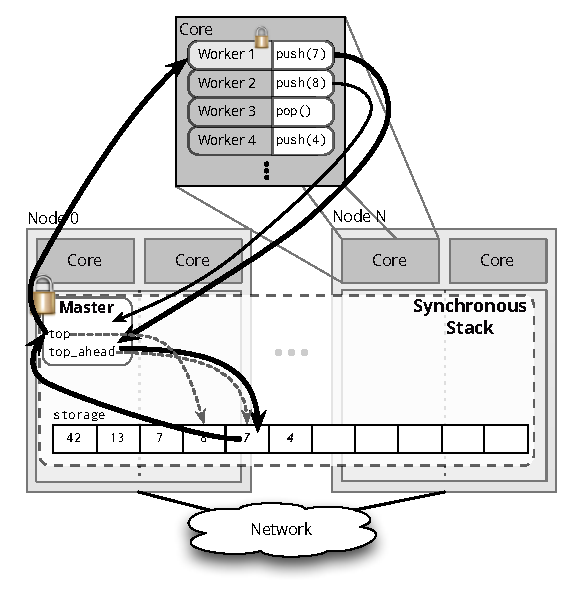
\includegraphics[width=\textwidth]{figs/stack_nofc.pdf}
    \caption{\emph{Without flat combining.}
      To do its push, Worker 1 sends a message to synchronize with the master on Core 0 (1), which sends another message to write the value to the top of the stack (2), bumps the synchronized \texttt{top} pointer (3), and finally continues. Worker 2, and all other workers on all cores accessing the stack, must block at the master and wait for Worker 1 to complete its push before doing their operations (4).
    }
    \label{fig:stacknofc}
  \end{subfigure}%
  \hspace{0.05\textwidth}
  \begin{subfigure}[b]{0.43\textwidth}
    \centering
    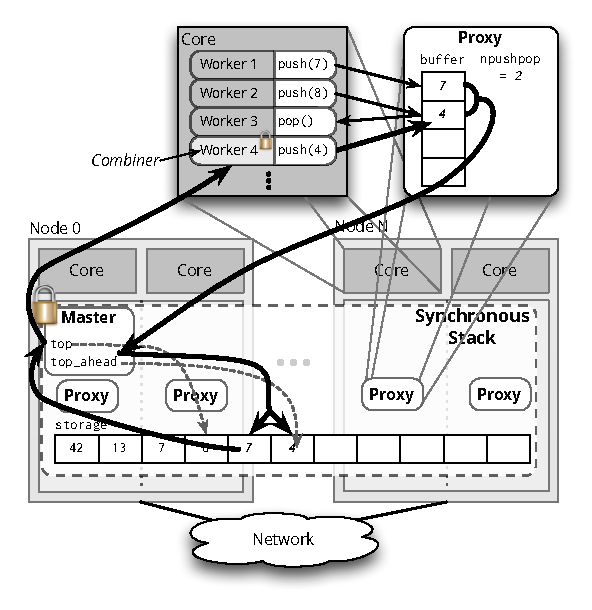
\includegraphics[width=\textwidth]{figs/stack_fc.pdf}
    \caption{\emph{Local flat combining.}
      Workers within the core add their requests to a local proxy object. Worker 3's pop matches with Worker 2's push, requiring no global communication (1). After combining locally, Worker 1 and 4's pushes remain, so Worker 4 becomes the core's combiner (2), sends a message to synchronize with the master (3), adds both new values to the global stack (4), bumps the top pointer and releases the lock on master (5), and finally wakes Worker 1 and continues (6).
    }
    \label{fig:stackfc}
  \end{subfigure}
  \caption{\emph{Global stack in Grappa} with and without \emph{flat combining}.}
  \label{fig:stack}
\end{figure*}

In a PGAS setting, and in Grappa in particular, the cost of global synchronization and the amount of concurrency is even greater than in shared memory. With thousands of workers per core, in a reasonably sized cluster there are easily millions of workers. This presents an opportunity for flat combining to pay off greatly, but also poses new challenges.

% a number of different choices are made when implementing flat combining. Because memory is physically distributed, locality must be made explicit. In addition, in Grappa there are orders of magnitude more concurrent threads (``workers'') accessing shared data structures. Typically around a thousand are needed per core to tolerate the latency of remote operations, so in a cluster of machines, there are easily millions of workers. Therefore, a different scheme for managing many threads is necessary.

To illustrate how flat combining can be applied to Grappa, we must first describe what a global data structure might look like. Figure~\ref{fig:stacknofc} shows a simple PGAS translation of the shared-memory stack from earlier. A storage array is allocated out of the global heap, so its elements are striped across all the cores in the system. One core is designated the ``master'' to enforce global synchronization, and holds the elements of the data structure that all concurrent accessors must agree on, in this case, the \texttt{top} pointer.

All tasks that want to access the global stack hold a \texttt{GlobalAddress} to the Master object. To perform an operation, the task invokes a custom delegate operation that, like the \texttt{read()} delegate described earlier, blocks the task until complete. Example code to do a \texttt{push} is shown in Figure~\ref{fig:push}, the task must send a message to the master to acquire the lock. If it succeeds, it follows the \texttt{top} pointer, writes its new value to the end of the stack, returns to bump the \texttt{top} pointer and release the lock, and finally sends a message back to wake the calling worker. All other workers performing operations block at the first message until the lock is released. Because of Grappa's user-level blocking mechanisms, blocked requests do not have to retry or busy-wait. However, all thousand workers on each core all perform this synchronization and serialize on the master core.

\paragraph{Centralized Combining.}
A first thought might be to directly apply the idea of flat combining to the serialization at the master node. The worker that acquires the lock on the master can walk through the requests of all the other workers waiting to acquire the global lock and perform combining on them. In the case of the GlobalStack, this would mean taking all of the push requests, matching them with the pops, and sending messages back to the remote workers with the results. Any leftover pushes or pops would be applied to the data structure, and another round of combining would begin. This approach, combining on the master, reduces traffic to the data structure storage, but the single ``master'' core must still process every single request. This approach will not scale when every other core can generate requests just as fast as the master can combine them.

\paragraph{Distributed Combining}
Instead of all workers on a core sending independent synchronization messages and putting the burden all on the master, what if each core did its own combining first, and synchronized with the master in bulk?
Distributing the combining to each core allows the majority of the work to be performed in parallel and without communication.
As with shared-memory combining, distributed combining improves locality, reduces the amount of global synchronization, and allows operations to be composed in data structure-specific ways for even greater performance.
% allows synchronization to happen in parallel on all the cores, 
% Flat combining in Grappa is about allowing synchronization and  distributing synchronization 
% In a way, Grappa's automatic message aggregation is already trying to reduce synchronization traffic; however, the generic mechanism for serializing and packing has a cost, and in the end, the operations must still serialize on the master.
% Flat combining is about ``teaching'' it how to more efficiently perform many operations remotely in certain special cases.

% In order for workers to cooperate locally, a local ``proxy'' object is allocated in the core-private heap. This proxy serves as the 

In distributed flat-combining, each core needs its own publication list to track all of its outstanding operations to be performed on the global data structure. In Grappa, this takes the form of a local \emph{proxy} object allocated from the core-local heap.
Conceptually, workers add their requests to the local publication list, one is chosen to do the combining, and the rest block until their request is satisfied.
However, because workers are scheduled cooperatively, each worker has atomic access to the local proxy ``for free'', so an explicit publication list is unnecessary.
Instead, each worker performs its own combining, pushing the 
, and blocks if it was unable to satisfy its request immediately. Figure~\ref{fig:stackfc} shows how in the global stack example, pushes and pops can be matched locally, avoiding global synchronization for those operations.

After all local combining has been done, one requesting worker is chosen to perform the combined operation globally. In the same figure, Worker 4 becomes the combiner and performs much the same synchronization as in the un-combined case, but is able to push multiple elements with one synchronization. As in the uncombined case, the global lock must still be acquired, and concurrent combined requests must still block and serialize on the master, though a technique later will describe how flat combining can be applied here, too. Combining in this way allows synchronization to be distributed and performed in parallel, coarsening the granularity of the actual global synchronization and reducing the amount of serialization that occurs.

% In most cases, this means communicating with whichever core holds the ``lock-protected'' field that maintains sequential consistency. In the case of a global stack, this is the ``master'' \emph{top} pointer which must be incremented on pushes and decremented on pops. On the core where global synchronization is occurring, there must be synchronization between the multiple synchronization requests arriving from other cores.

% At this point we have traded off one remote synchronization per operation for an additional local synchronization per operation and some number fewer remote synchronizations (depending on the amount of combining that occurs). This would likely result in a net benefit due to local synchronization being inherently cheaper. However, because of the way the Grappa runtime schedules computation, it is actually possible to get the correct mutual exclusion/atomicity without any additional synchronization overhead.

% By design, each core in Grappa operates independently of the other cores. Workers are scheduled cooperatively, so each worker can assume atomicity until it performs an operation that yields to the scheduler, such as a remote call. Therefore workers within a core can cooperate without any explicit synchronization operations requiring memory fences. This allows them to publish requests to the local proxy very inexpensively, eliminating the need for a complex synchronization-amortizing queue. This has the added benefit that there will be no unused publication records, which could have become a problem with thousands of workers. Further, remote operations are processed through the same cooperative-multithreading scheduler on the remote side, so combined operations are trivially serialized and atomic.

\paragraph{Sequential Consistency}
The sequential consistency guarantee is that within a task, operations will be in task order, so to enforce ordering between operations in different tasks, one task must perform an operation that another one can observe. An example is shown in Figure~\ref{fig:sync}.\TODO{make sync example}
The Grappa memory model is in the style of the C++ memory model~\cite{boehm:drf0,N2480,N2800} memory model (guaranteeing sequential consistency for data-race free programs). Being conservative, delegate operations block the calling worker until they have completed globally, ensuring they can be used for synchronization. As such, delegate operations within a task are guaranteed to be globally visible in program order.
Because it is not immediately obvious that this distributed version of flat combining preserves sequential consistency, here we will make arguments for why it does.

% \begin{itemize}
%   \item Block the calling worker until the operation is guaranteed to have a valid global order.
%   \item Local combining must not allow workers to observe a different order than is committed globally.
% \end{itemize}
To preserve sequentially-consistent semantics for flat-combined operations, they must obey a consistent global order.
To start with, local combined operations must have a serializable order among each other; this is unchanged from shared-memory flat-combining, and is trivially true due to the atomicity enabled by cooperative multithreading.
When combined operations are applied globally, they are serialized at a particular core that owns the synchronization (the ``master'' core for the Queue and Stack, or the corresponding hash cell for the Set and Map). The global order, then, is essentially the concatenation of the cores' sequential orders.
For this ``concatenation'' to be valid, the order observed by workers during local combining must be the same as what can be observed globally as operations are committed.

In the case of the Stack and Queue, this guarantee comes from applying a batch of push or pop operations atomically in a contiguous block on the global data structure. The second level of combining at the master preserves this as well by only allowing updates to proceed when they will not conflict and blocking all of them until they have completed.
Matching pushes and pops locally is one exception to the rule that operations must block until globally committed. Because a pop ``destroys'' the corresponding push, these operations together are independent of all others and can conceptually be placed anywhere in a total global ordering, so they can be safely matched locally.

The correctness of combining set and map operations is more nuanced.
Insert and lookup operations performed by different tasks are inherently unordered unless synchronized externally.
Therefore, a batch of these operations can be committed globally in parallel.
If an insert finds that its key is already in the combiner, it does not need to send its own message. However, it must still block until that insert is done, otherwise it may assume that the key has been inserted and perform some other operation that requires the insert to have happened.
In the same way, lookups can piggy-back on other lookups of the same key.
It is tempting to allow a lookup to be satisfied locally by inspecting the keys to be inserted.
However, this allows the local order in which keys were inserted to be observed.
If this is allowed, then that same order must be respected globally, forcing each batch to ensure atomicity from all other cores' batches. This is prohibitively expensive, so a cheaper solution is chosen: lookups must get their values from the global data structure, but can be performed in parallel in the same way as inserts.

% (wrong!) A lookup can be satisfied locally provided that the insert it relies on is guaranteed to eventually be committed globally. This allows the task to continue. If it does another lookup to a different key that is satisfied locally, then that task has observed one particular ordering of the two inserts. When those inserts commit globally, they will proceed in parallel to their respective hashed locations. Another task could 

% The combining operations that are performed locally among requests on a single core must preserve the illusion of sequential order; this is unchanged from shared-memory flat-combining. When combined operations are applied globally, they are serialized at the ``master'' core for a given synchronization context. The global order is essentially the concatenation of each core's batch of serialized accesses.
% In the case where operations are satisfied locally (by matching up with other local operations), by definition these must be independent of other operations, so they can conceptually be placed anywhere in the global ordering (or even ignored completely in the global ordering).

% In the spirit of the Data-Race-Free-0 Model (guaranteeing sequential consistency for data-race free programs), operations on the global data structure are considered to be made atomic by a conceptual global ``lock'' on the data structure. 

These requirements only guarantee sequential consistency for a data structure in isolation. Atomicity and data race freedom in the case of multiple data structures must be guaranteed externally, just as in any multithreaded shared-memory program.

\section{Grappa FC Framework}
% One of the strengths of flat combining is that the same combining mechanism can be applied in multiple data structures. Each structure must only specify how its operations compose.
% Many different data structures can integrate flat combining into their operation using the same delegation mechanism, making it easier to implement concurrent data structures.
In order to leverage the flat-combining paradigm in Grappa, we implemented a generic framework which can be used to improve performance for a number of global data structures. The FC framework handles the common problems of managing the combiners, handling worker wake-ups, and maintaining progress. When hooking into the framework, each data structure implementation need only define how to combine operations and globally commit them.

% As discussed before, Grappa's distributed combining takes a different approach to expressing how operation locally  flat combining design takes a different approach to performing 
The Grappa FC framework takes a different approach than the original flat-combining work for expressing how operations combine. As mentioned before, the local ``publication list'' is trivial to access atomically in Grappa due to workers being cooperatively scheduled.
Instead, in the Grappa FC Framework, a \emph{proxy} object is instantiated ahead of time on each core and each worker merges its update into that structure before blocking or becoming the combiner.
% In the original work, an explicit publication list is built up, and when the combiner scans over the list, it has a structure that it uses to accumulate requests in a logical way. In the case of the stack, for instance, it is a thread-local stack, which it can use to immediately match up pushes and pops. In the Grappa implementation, each worker's actions are atomic anyway, so rather than creating an explicit request list, the combiner object (or \emph{proxy}) is instantiated ahead of time for the data structure, and each worker does its own local combining into that structure before blocking. This reduces the space blowout of a large dynamically-sized publication list (with associated caching issues), and does not overly affect the expression of combining.
In this style, each global data structure must define the following:
\begin{enumerate}
  \item A local \emph{proxy} data structure for tracking updates to the global structure.
  \item \emph{Combining methods} that operate on the local proxy.
  \item A \emph{sync} method that globally commits the proxy's state.
\end{enumerate}
An example proxy declaration for the GlobalStack is shown in Figure~\ref{fig:proxy}.

\begin{figure}[t]
\centering
\begin{lstlisting}[style=grappa]
class GlobalStack {
  GlobalAddress<T> top;
  Grappa::Mutex lock;
};

void push(GlobalAddress<GlobalStack> stack, T e) {
  // perform operation on the stack's master core
  delegate::call(stack.core(), [stack,e]{
    // force other operations to wait
    stack->lock.acquire();
    // do remote write to the top of the stack
    // (so other workers may interleave)
    delegate::write(stack->top, e);
    // bump the top pointer
    stack->top++;
    stack->lock.release();
  }); // blocks until response arrives
}\end{lstlisting}
\caption{Snippet of code for pushing to a global stack (without flat combining).}
\label{fig:push}
\end{figure}

\begin{figure}[t]
\centering
\begin{lstlisting}[style=grappa]
class GlobalStackProxy : Grappa::FCProxy {
  // pointer to data structure master
  GlobalAddress<GlobalStack> master;
  
  // local state for tracking pushes and pops
  T  pushed_values[1024];
  T* popped_results[1024];
  int npush, npop;

  // Combining Methods 
  // (either match locally or block for results)
  void push(T val);
  T pop();
  
  // Global sync (called by FC framework)
  void sync() override {
    if (npush > 0) {
      // on master, acquire lock and return GlobalAddress to the top of the stack
      auto top = delegate::call(master.core(),[=]{
        master->lock.acquire();
        return master->top;
      });
      // copy values to top of stack
      Grappa::memcpy(top, pushed_values, npush);
      // release lock at the master core
      delegate::call(master.core(),[master,npush]{
        master->top += npush;
        master->lock.release();
      });
    } else if (npop > 0) {} //...elided for space
  }
};
\end{lstlisting}
\caption{Snippet of the Proxy object for the GlobalStack. The code to synchronize pushes should resemble that from Figure~\ref{fig:push} but for multiple elements.}
\label{fig:proxy}
\end{figure}

With this data structure-specific proxy object, the FC framework does the bookkeeping to block and wake Workers, deliver results, manage when to synchronize, and choose the combiner.
The FC framework is responsible for ensuring that all of the combined operations eventually get committed. There are a number of ways progress could be guaranteed, but one of the simplest is to ensure that as long as there are any outstanding requests, at least one worker is committing a combined operation.
When that combined operation finishes, if there are still outstanding requests that have built up in the meantime, another blocked worker is chosen to do another combined synchronization.

One could imagine other synchronization policies that would ensure progress but allow more combining to occur before synchronizing. For instance, local combining could continue until all workers are blocked. However, this would require the flat-combining framework to track the activity of the workers on a core, and additionally would add latency unless the system saved enough active workers to tolerate the latency of the global commit action. As it is, the one-in-flight policy implemented performs well, and does not require any coupling with the Grappa scheduler. Exploration of other policies is left for future work.

While a combining operation is in flight, new requests are likely to continue to accumulate. The framework transparently wraps the proxy object so that when it starts a sync on one, it can direct requests to a fresh combiner. It is important to note that combiners must start out fresh each time---it would be unsound for them to ``remember'' the previous updates and attempt to combine locally with them.

% The flat combining framework transparently wraps the \emph{proxy} object. Behind this layer of indirection, it manages multiple copies of the proxy so that, as discussed above, there is always at least one being committed and one to receive additional combining operations.

% explain simple non-combined global data structures in Grappa section...

\subsection{Global Stack and Queue}
Figure~\ref{fig:proxy} shows an excerpt from the definition of the proxy object for the Grappa GlobalStack. The proxy tracks pushes locally in the \texttt{pushed\_values} array. When \texttt{pop()} is called, if there are pushes in the local array, it immediately takes the value and wakes the last worker to push. Otherwise, it adds a pointer to a location on its stack where the \texttt{sync} operation, will eventually write the result. Because of local matching, when a Stack proxy is synchronized, it will have either all pops or all pushes, which makes the implementation of sync straightforward. Note that the operation to synchronize a batch of pushes looks almost identical to the code to do a single push from Figure~\ref{fig:push}.

The GlobalQueue has nearly the same implementation as the stack, but is unable to match locally, so \texttt{sync} first does the pushes, then does the pops.

\subsection{Global Set, and Map}
The Grappa GlobalSet uses a simple chaining design, implemented with a global array of cells (allocated from the global heap), which are partitioned evenly among all the cores, and indexed with a globally-agreed hash function. Our flat-combining version supports both \texttt{insert} and \texttt{lookup}. To track all of the keys waiting to be inserted, we use the hash set implementation from the C++11 standard library (\texttt{std::unordered\_set}). Similar to the case with pops, for lookups, we must keep track of pointers for where to put the results of lookup operations, which the proxy does with a hash map (again from the C++ standard library) from keys to a list of pointers. As discussed in Section~\ref{sec:sc}, matching lookups with inserts locally would force a particular sequential order, so instead we only allow matching inserts with inserts and lookups with lookups. This allows \texttt{sync} to simply issue all of the inserts and lookups in parallel and block until all have completed.

Our implementation of the GlobalMap matches that of the Set, but of course stores values of a given type. This does not change the requirements of the proxy except that the return values of lookups must be a copy of the value rather than just a boolean.


\section{Evaluation}
\label{sec:evaluation}

The goal of our evaluation is to show that the core pieces of the \Grappa
runtime system, namely our tasking system and the global memory/communication
layer work as expected and together are able to efficiently run irregular
applications. We evaluate \Grappa in three basic steps:

\begin{itemize}

\item We present results that show that the \Grappa runtime is able to sustain
very high concurrency rates and the communication layer is able to sustain a
very high rate of global memory operations. We also show the performance of a
graph kernel that stresses communication and concurrency together.

\item We show how some popular irregular applications running on \Grappa
compare to the Cray XMT and hand-tuned MPI code.

\item We finish with a characterization of system behavior, including
profiling where execution time goes, how aggregation affects message size and
rates, how global memory and work stealing behaves.

\end{itemize}

\subsection{Basic \Grappa Mechanisms}
\label{eval:basic}

\paragraph{User-level context switching.}

As discussed earlier, fast context switching is at the heart of \Grappa's
latency tolerance abilities. We assess context switch overheads using a simple
microbenchmark that has a configurable number of workers, where each worker 
just increments values in a large array. 

\begin{figure}[ht]
    \begin{center}
      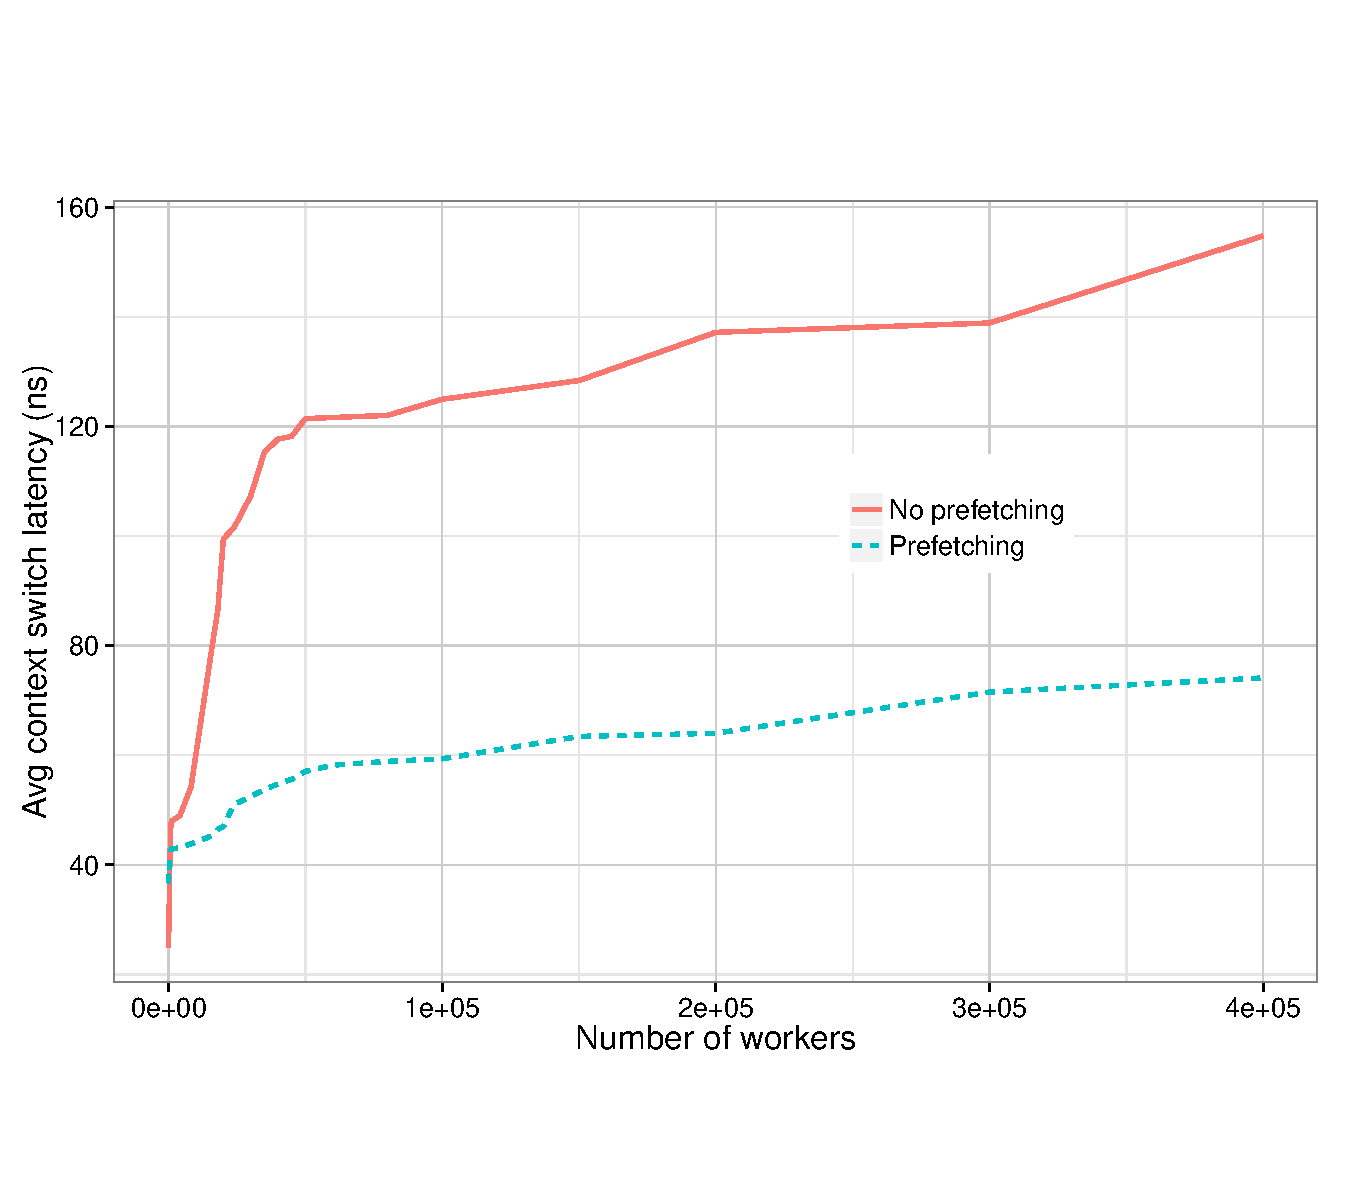
\includegraphics[width=0.5\textwidth]{figs/context_switch_time.pdf}
    \end{center}
    \caption{Average context switch time with and without prefetching.}
    \label{fig:context-switch-exp}
\end{figure}

Figure~\ref{fig:context-switch-exp} shows the average context switch time as
the number of workers grow. There are two important takeaway points from these
data. Context switch time for the number of workers we use ($~$1K workers) is
on the order of 50 ns; and prefetching has significant impact on context
switch time. And context switch time does not grow significantly with the
number of workers --- even with one-half million workers, context switch
is around 75ns.

We also measured (not in the plot) the \emph{rate} of context switch for all
cores in a node, which showed that our rate is limited by off-chip memory
bandwidth. Each context is 4 cache lines (1 for the worker struct and 3 for
stack data), leading to 8 cache line transfers per context switch
(write the previous context, read the next in). The off-chip bandwidth of a
single socket in our system is 270M cache lines per second, which implies that
we can sustain at most 34M context switches per second per socket, which is
almost exactly what we sustain.

In summary, our context switch engine is able to efficiently sustain very high
concurrency and as we will show later, the amount of concurrency sustained is
sufficient the latencies \Grappa needs to hide.

\paragraph{Global memory and communication.} We measure the performance of
\Grappa's global memory and communication layers using a faithful
implementation of the giga updates per second (GUPS) benchmark.
Read-modify-write updates are dispatched at random to a large array. This
benchmark stresses the communication layer of \Grappa separately from the
scheduler, because only a single worker is used per system node.
Figure~\ref{fig:grappa-gups} shows that \Grappa is able to sustain well over a
billion updates per second with 64 nodes. This compares very favorably to
published results~\cite{gups} for other high-end HPC systems.


\begin{figure}[ht]
    \begin{center}
      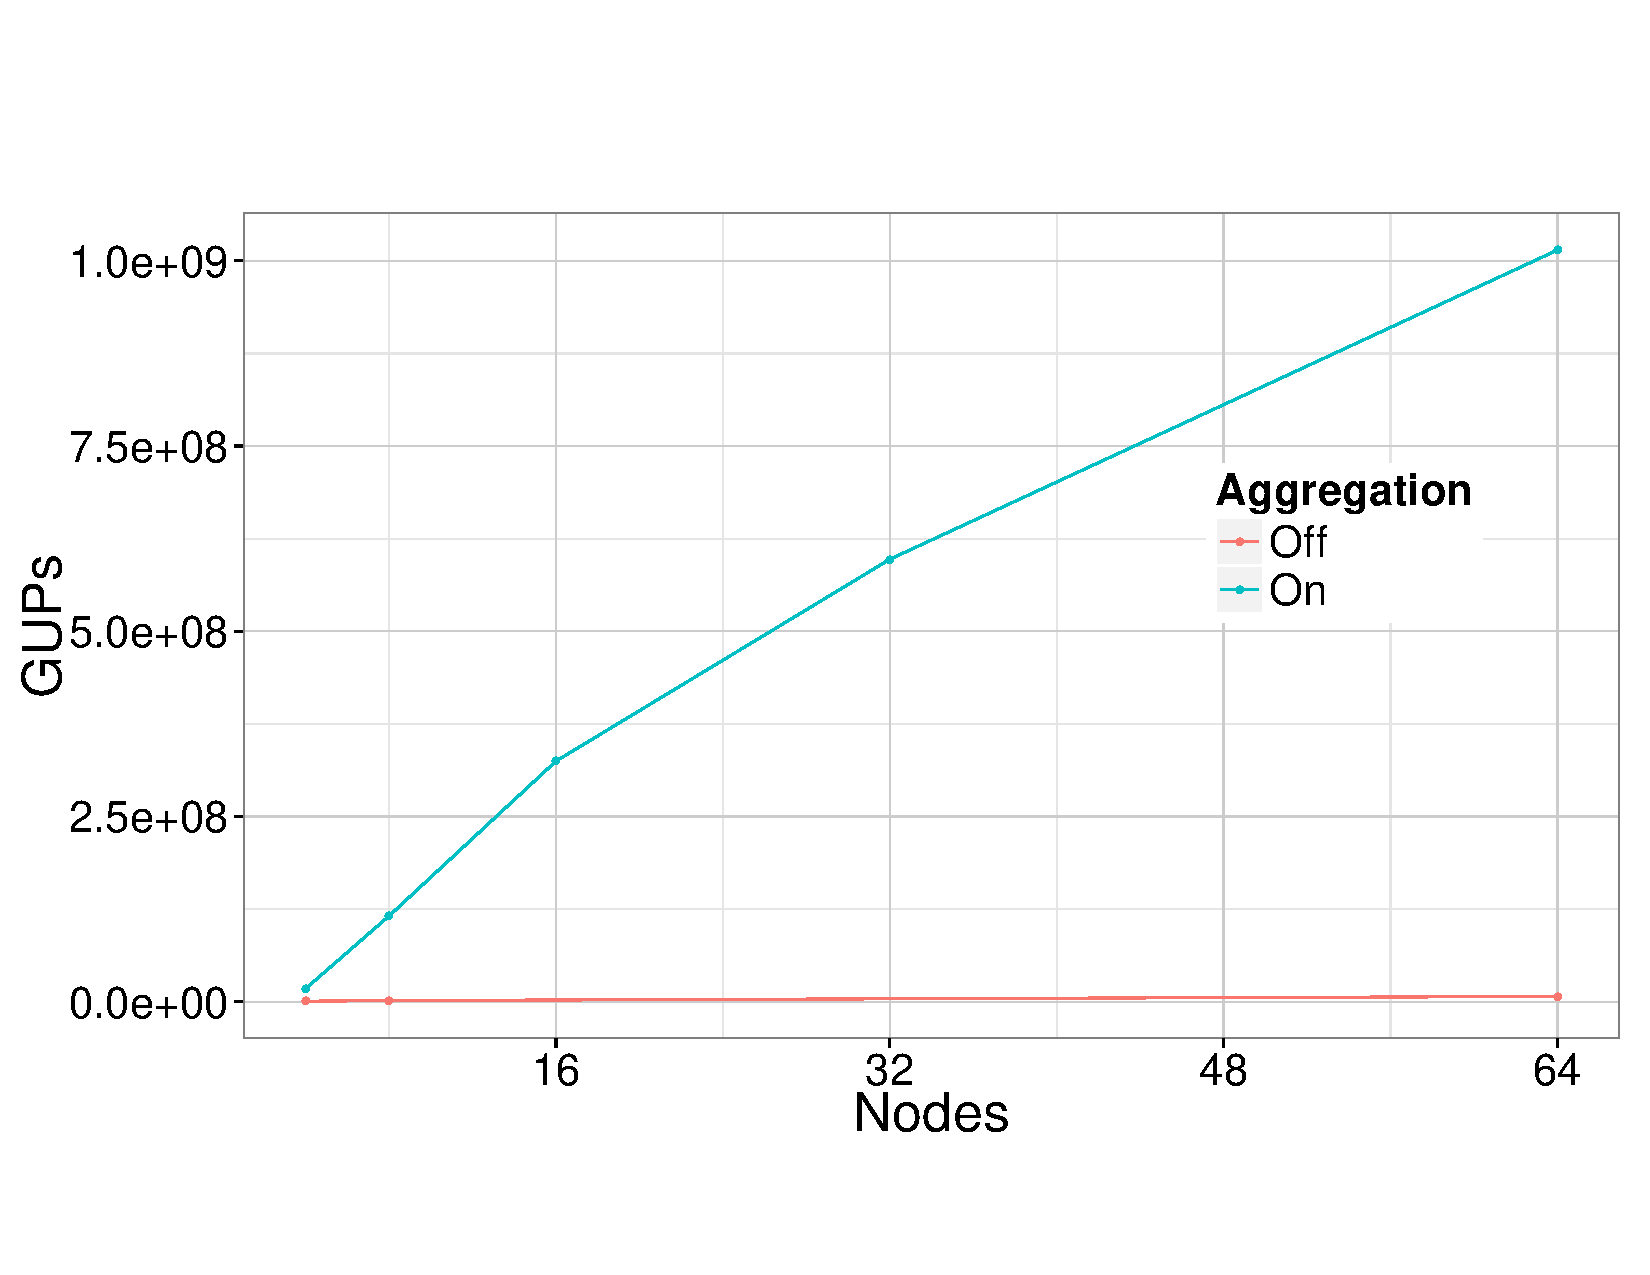
\includegraphics[width=0.5\textwidth]{results/gups/gups.pdf}
    \end{center}
    \caption{GUPS (giga updates per second) for \Grappa as the number of nodes grows.}
    \label{fig:grappa-gups}
\end{figure}

\paragraph{Putting it all together with Unbalanced Tree Search in
    memory (UTS).}
We now show the overall performance of \Grappa running UTS.
Figure~\ref{fig:grappa-uts}. The point of this experiment is to
demonstrate whether \Grappa's context switching and communication layers can in fact
be used together, while balancing workload, to run an irregular application efficiently. 
We look at two classes of trees, T1x and T3x, from the
original benchmark. T1x trees are very shallow and wide, while T3x
trees are very deep. When the access to each vertex is a random
access, the critical path to search T3x trees is very long. On such
trees, we do not expect there to be sufficient concurrency for any
system, including \Grappa, to achieve high throughput. \TODO{plot it
    if time}. To verify this, at the 16-node data point, the average active tasks per
core over the search is 775 and 13 for T1XL and T3L, respectively.

\begin{figure}[ht]
    \begin{center}
      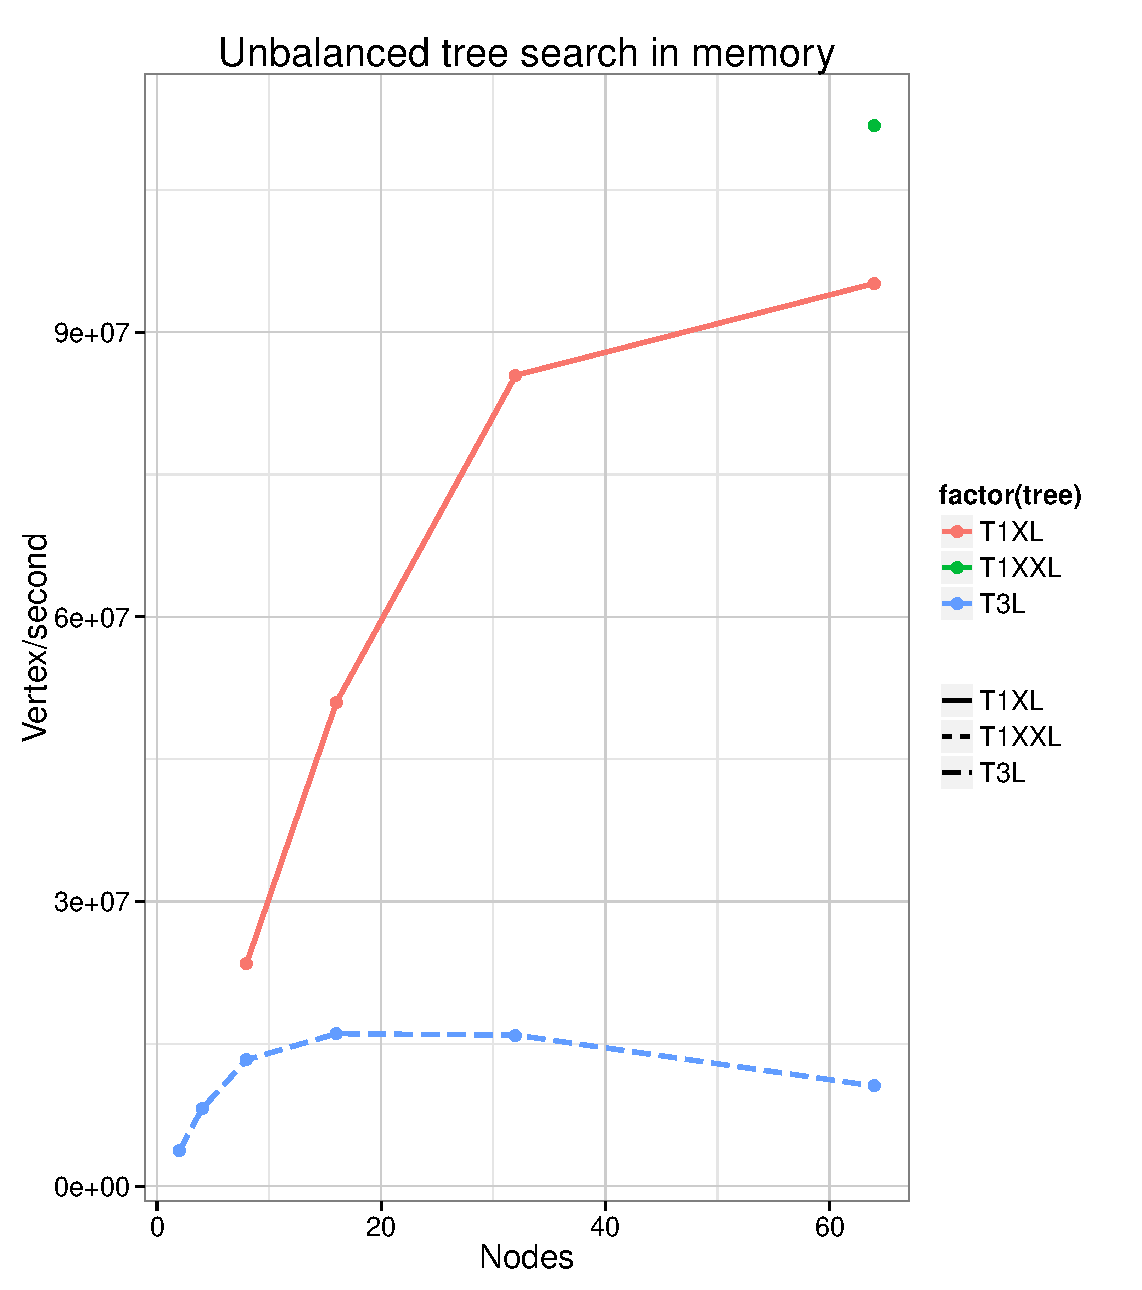
\includegraphics[width=0.5\textwidth]{figs/uts_scale.pdf}
    \end{center}
    \caption{Vertices per second in UTS on \Grappa as the number of nodes grows.}
    \label{fig:grappa-uts}
\end{figure}


\subsection{Comparing \Grappa to Other Systems}

In order to put \Grappa's performance into a general context, we compare it
with XMT running BFS, PageRank, IntSort, GUPS and UTS. Since XMT is a
different hardware platform, we also compare \Grappa with hand-tuned MPI
versions of BFS and GUPS running on the same hardware. Finally, we also
compare it with UTS written for UPC. We run all experiments with 64 nodes.

\begin{figure}[ht]
    \begin{center}
      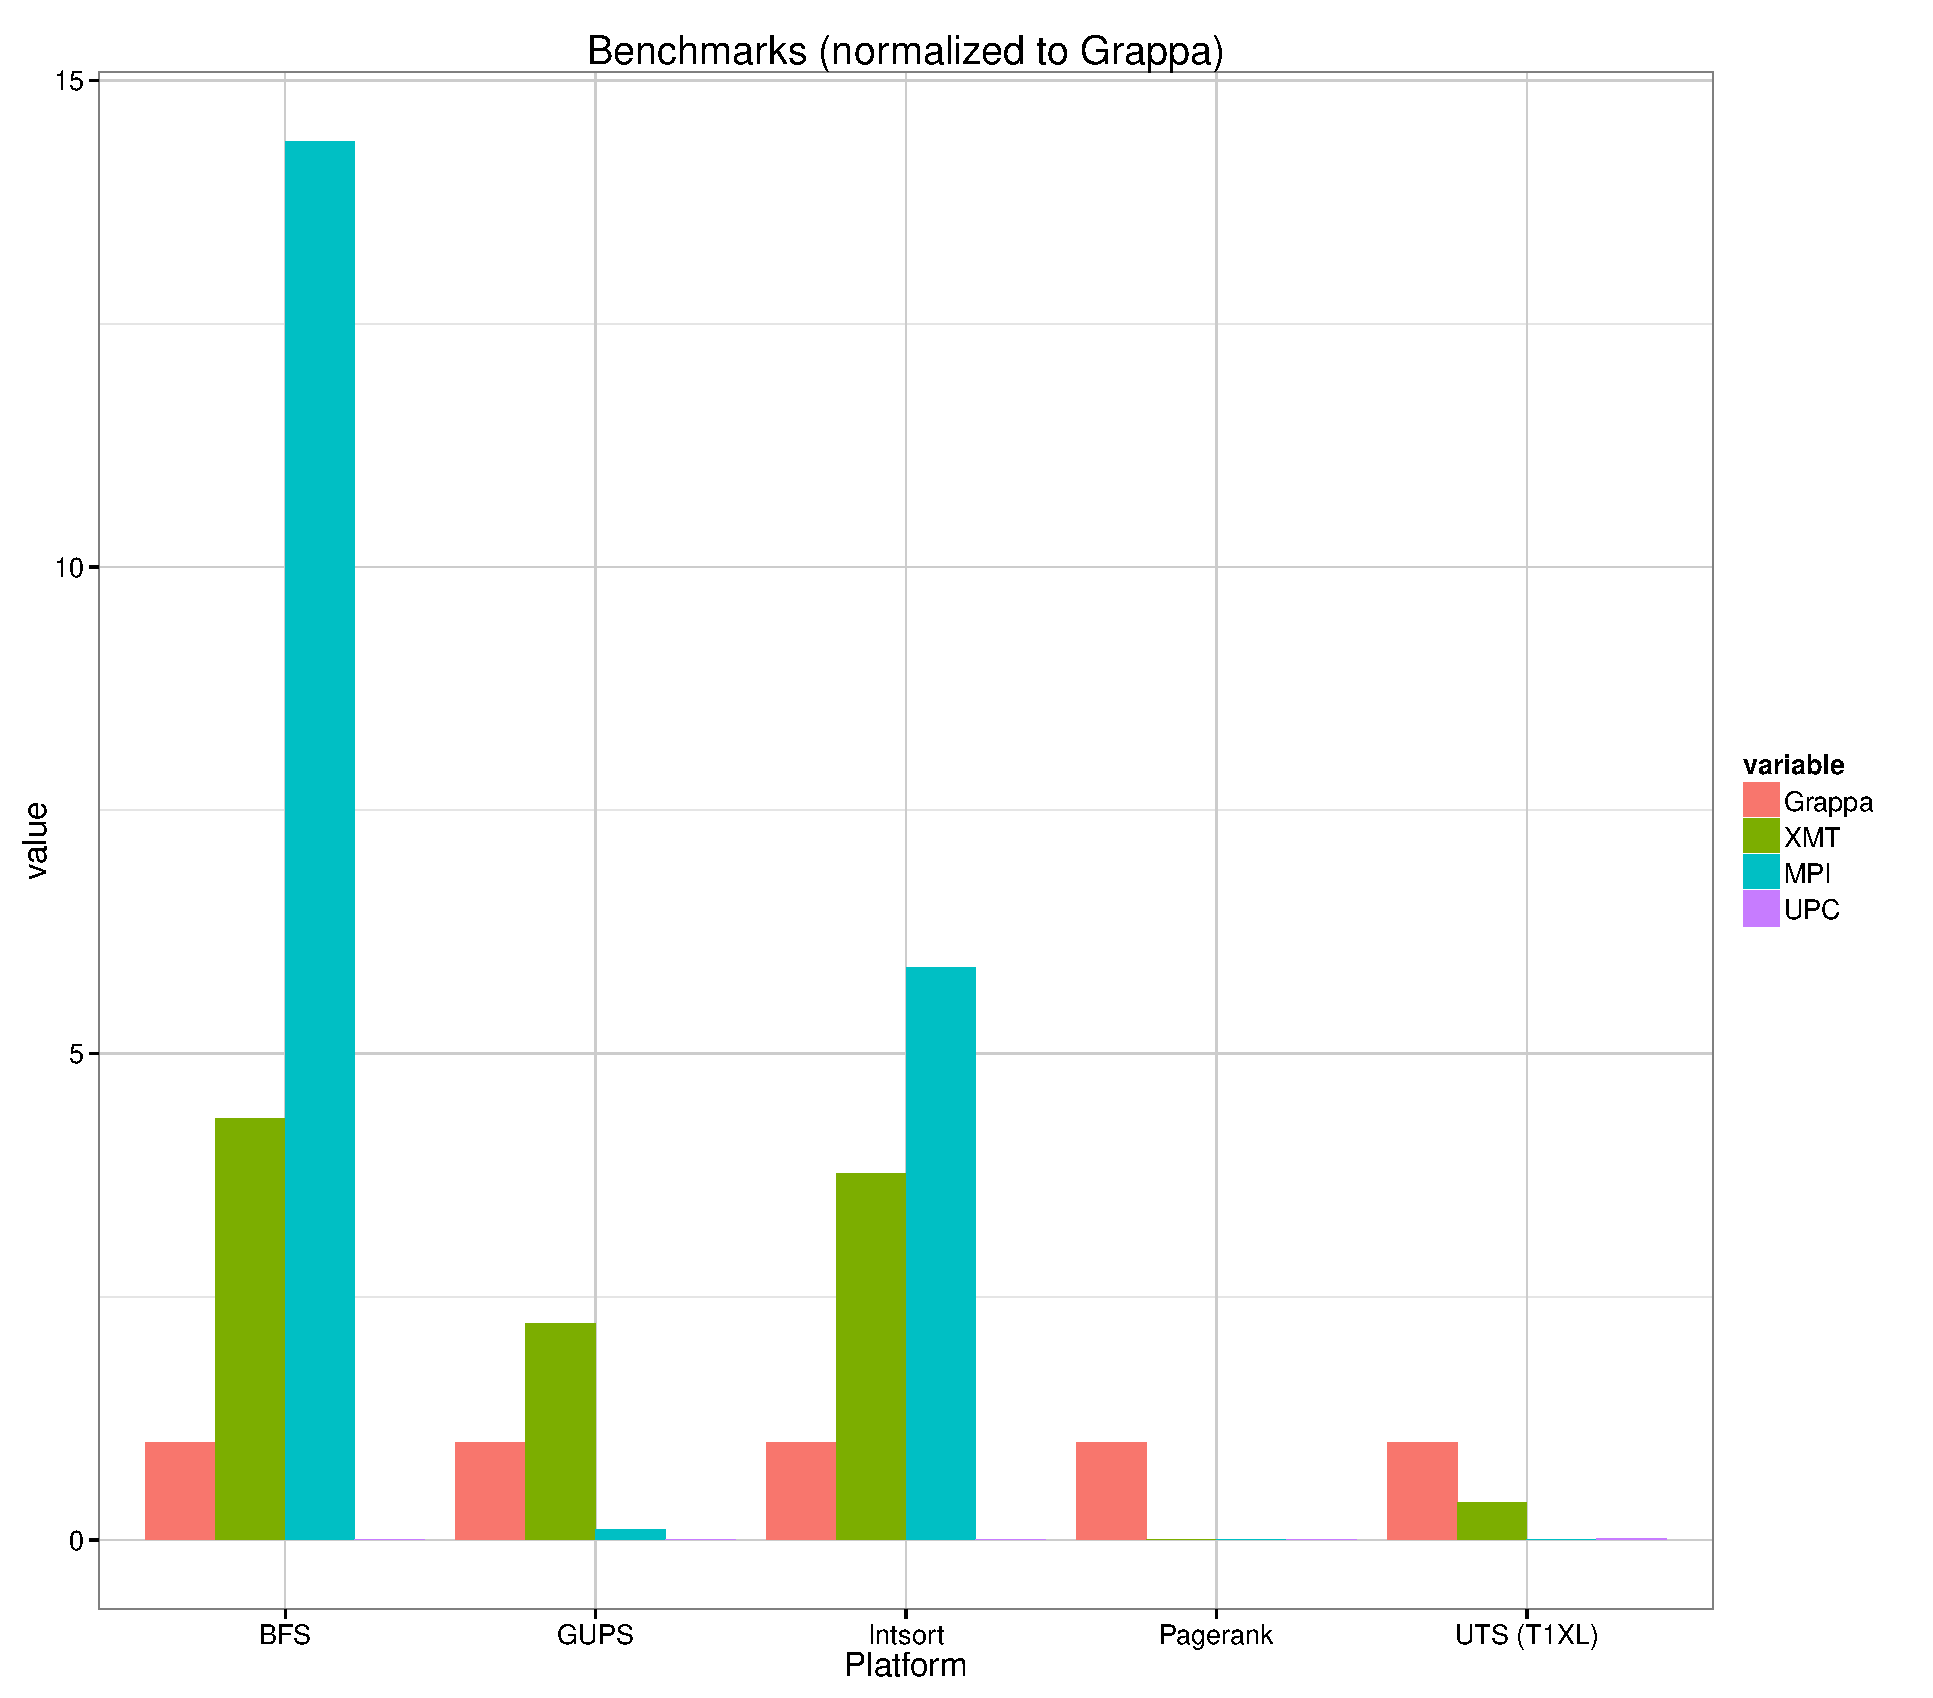
\includegraphics[width=0.5\textwidth]{results/benchmarks.pdf}
    \end{center}
    \caption{Comparing \Grappa with XMT, hand-tuned MPI and UPC.}
%bar chart, one set of bars per benchmark, one bar per system. runtime normalized to grappa.
    \label{fig:grappa-comparisons}
\end{figure}

Figure~\ref{fig:grappa-comparisons} shows the results. Overall, \Grappa is
within striking distance of XMT and UPC performance. However, it underperforms
compared to hand-tuned MPI. Nevertheless, this comparison needs to be taken
with a grain of salt for several reasons. First, we have not spent as much
time tuning \Grappa's implementations. This is supported by inspecting the BFS
MPI implementation we used, which clearly shows that it employs a lot of
algorithmic-specific optimizations. In fact, some of these optimizations
resemble some of what \Grappa does automatically, like message aggregation.
Second, the GUPS results presented earlier suggests that \Grappa performance
can do a lot better. \TODO{update this once we have more results. }

\subsection{Characterization}

\paragraph{Where execution time goes.}


\begin{figure}[ht]
    \begin{center}
      \begin{tabular}{c|c c c c}
        Benchmark     & Comm & User & Idle & Sched \\ \hline
        GUPS          & 6.60  & 42.94   & 47.74 & 2.80 \\
        BFS           & 54.84 & 30.90   & 10.94 & 3.43 \\ 
        Intsort       & 34.28 & 42.00   & 21.31 & 2.47 \\ 
        UTS           & 40.57 & 56.52   &  1.21 & 1.73 \\
        Pagerank      & 76.79 & 20.71   &  0.06 & 2.50 \\
      \end{tabular}
    \end{center}
    \caption{\Grappa\ execution time profile, in percent.}
%bar chart, one set of bars per benchmark, one bar per system. runtime normalized to grappa.
    \label{fig:grappa-profile}
\end{figure}

\TODO{PAGERANK:
    Without parallelizing the dot product, \Grappa cannot achieve
high utilization of workers proportional to the size of the data set.
Also mention that the cost of this is contention at the target
elements of vector.  The other parts of pagerank are super fast
(table?)
}

\paragraph{Message size and latency.}
Distribution if possible. With and without aggregation. 

\begin{figure}[ht]
    \begin{center}
      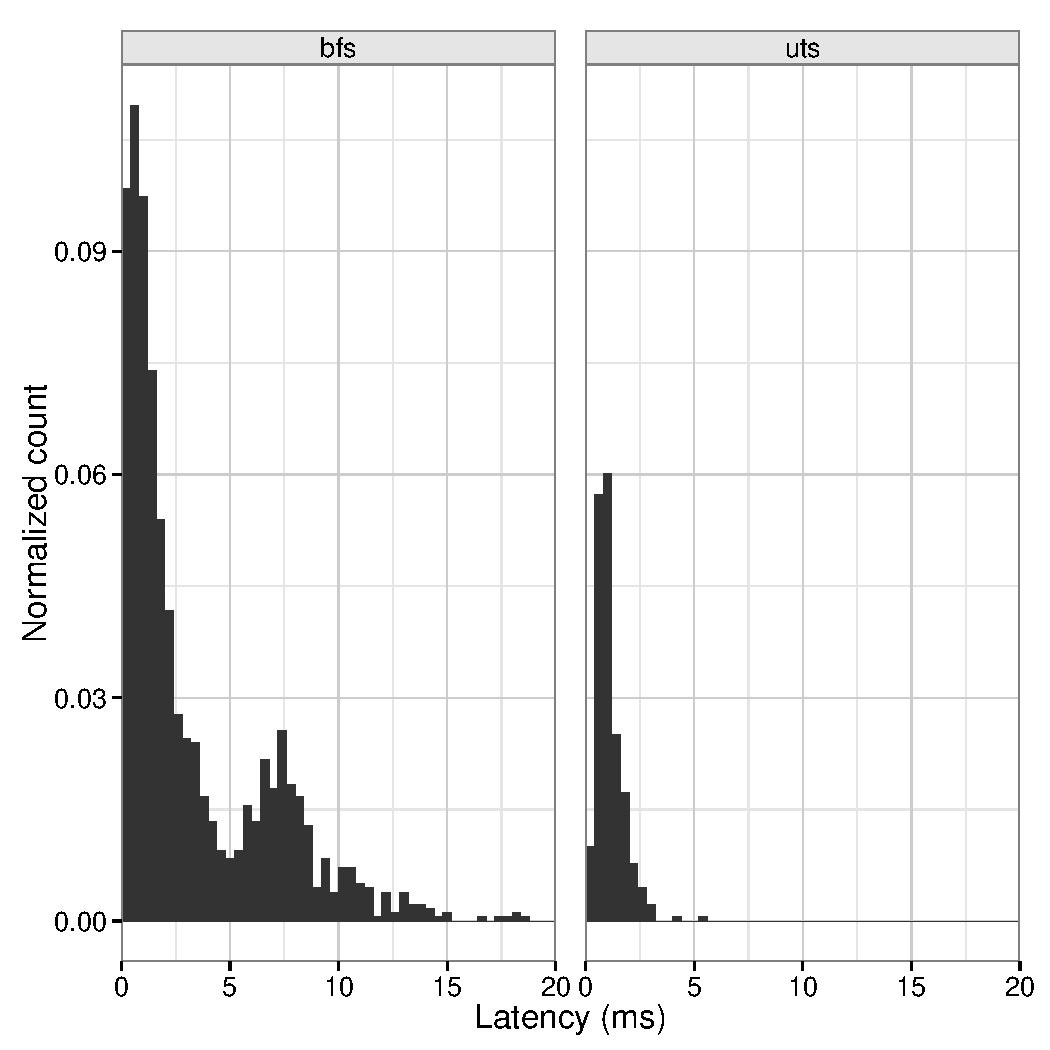
\includegraphics[width=0.5\textwidth]{results/histograms/latency_cmb.pdf}
    \end{center}
    \caption{Round-trip latency of delegate operations.}
%bar chart, one set of bars per benchmark, one bar per system. runtime normalized to grappa.
    \label{fig:grappa-latency}
\end{figure}

\begin{figure}[ht]
    \begin{center}
      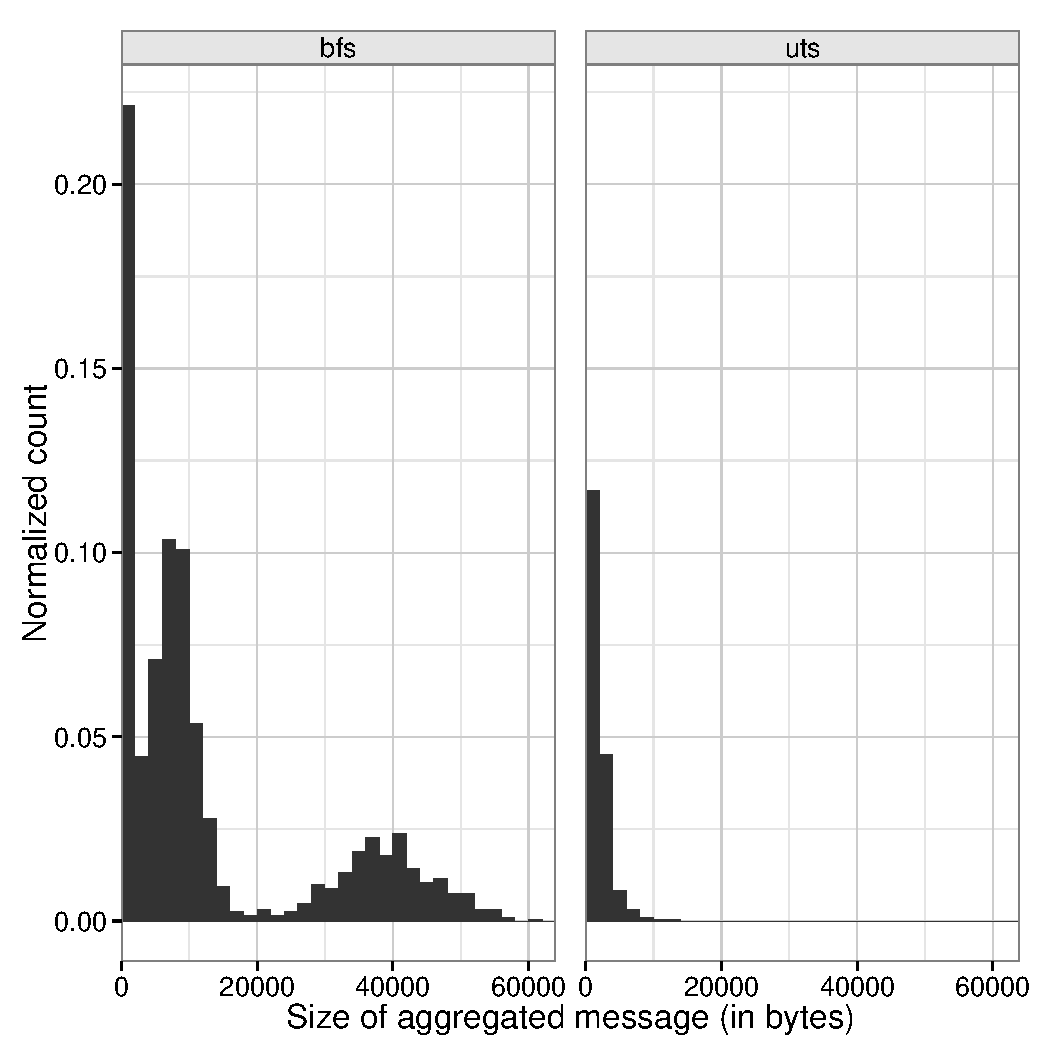
\includegraphics[width=0.5\textwidth]{results/histograms/rdma_bytes_sent_histogram_cmb.pdf}
    \end{center}
    \caption{Distribution of aggregated message sizes.}
%bar chart, one set of bars per benchmark, one bar per system. runtime normalized to grappa.
    \label{fig:grappa-message-size}
\end{figure}


\paragraph{Frequency of remote requests.}

\paragraph{Work stealing behavior.}
Performance loss of not having stealing. Ratio of \# of steals over total \# of task spawns. UTS needs stealing to work. 
















%%%%%%%%%%%%%%%%%%%%%%%%%%%%%%%%%%%%%% OLD %%%%%%%%%%%%%%%%%%

\comment{


Our evaluation begins with presentation of microbenchmark results, establishing
the intrinsic potential of \Grappa to provide random access bandwidth and latency tolerance. 
Next, we present application results, both for \Grappa and for other paradigms, as well
as comparing against the Cray XMT.  Finally, we present the impact of increased aggregation delay
on \Grappa results, thus exploring robustness to network scale.

\subsection{Microbenchmark Results}

\subsubsection{Random Access}
\TODO{Random access feed forward results on \Grappa.  optional: Results we measured for XMT.  Cite MPI results}
\subsubsection{Latency Tolerance}
\TODO{Simple ping test results -- eg, MPI ping, not the full blown aggregation ping test.  Random access blocking results on \Grappa.}
\subsubsection{Scheduling and Robustness}

\begin{figure}[ht]
    \begin{center}
      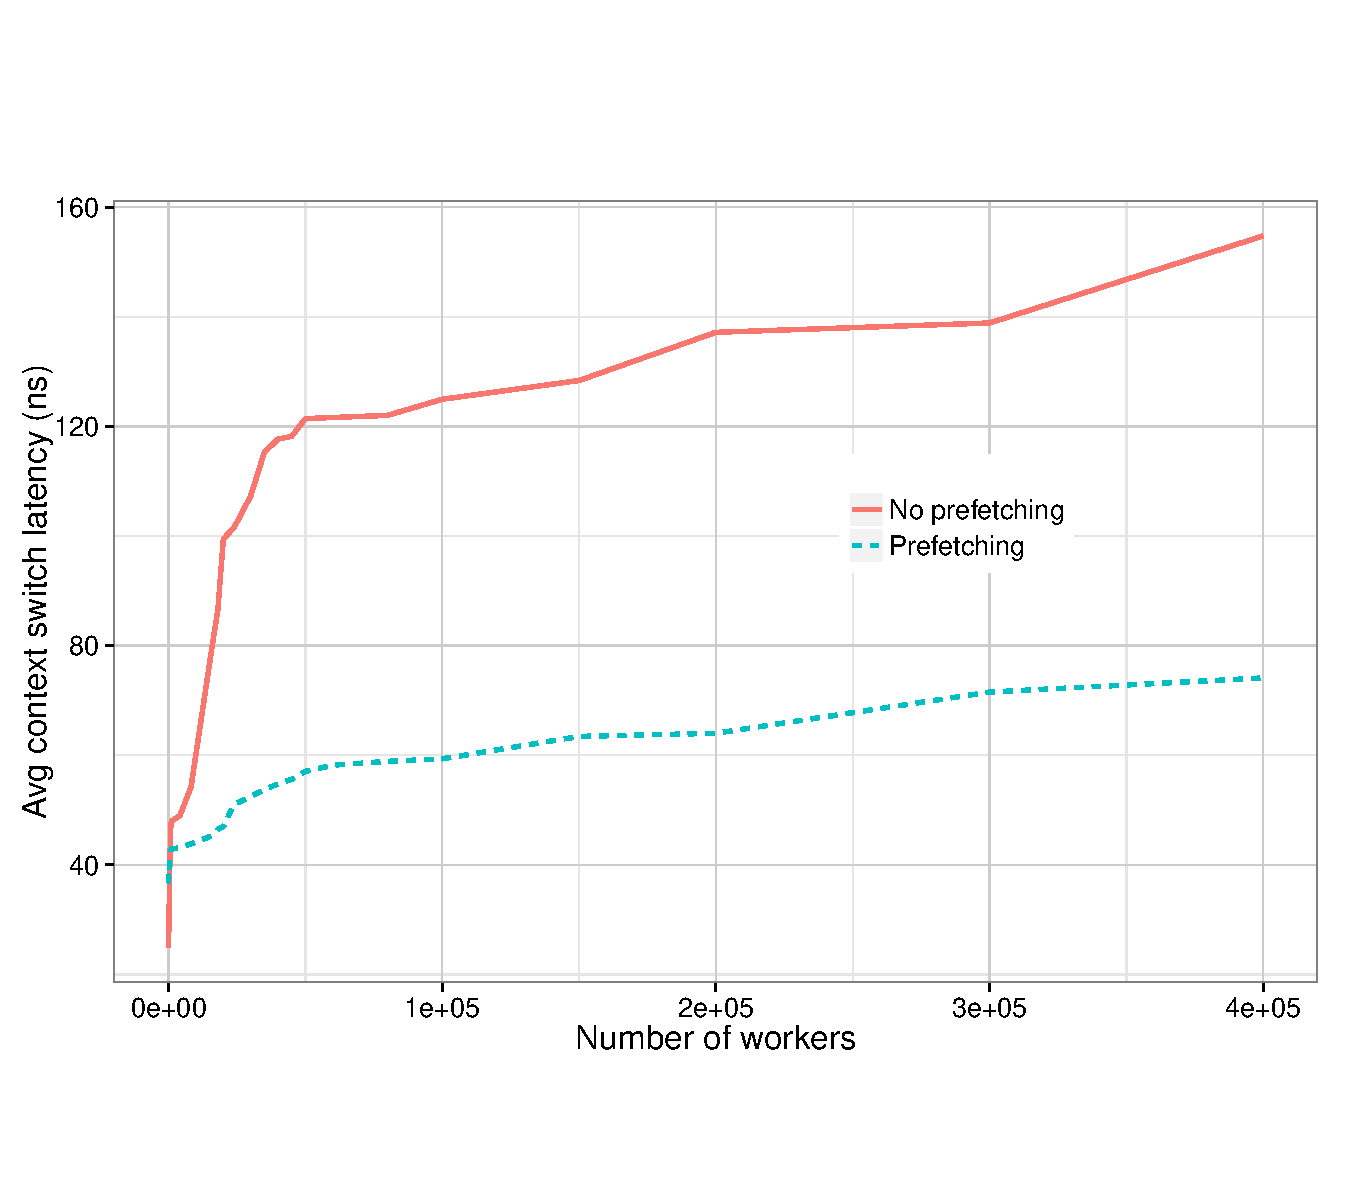
\includegraphics[width=0.5\textwidth]{figs/context_switch_time.pdf}
    \end{center}
    \caption{Average context switch time with 1 and 6 active cores,
        with and without prefetching.}
    \label{fig:context-switch-time}
\end{figure}

\begin{figure}[ht]
    \begin{center}
      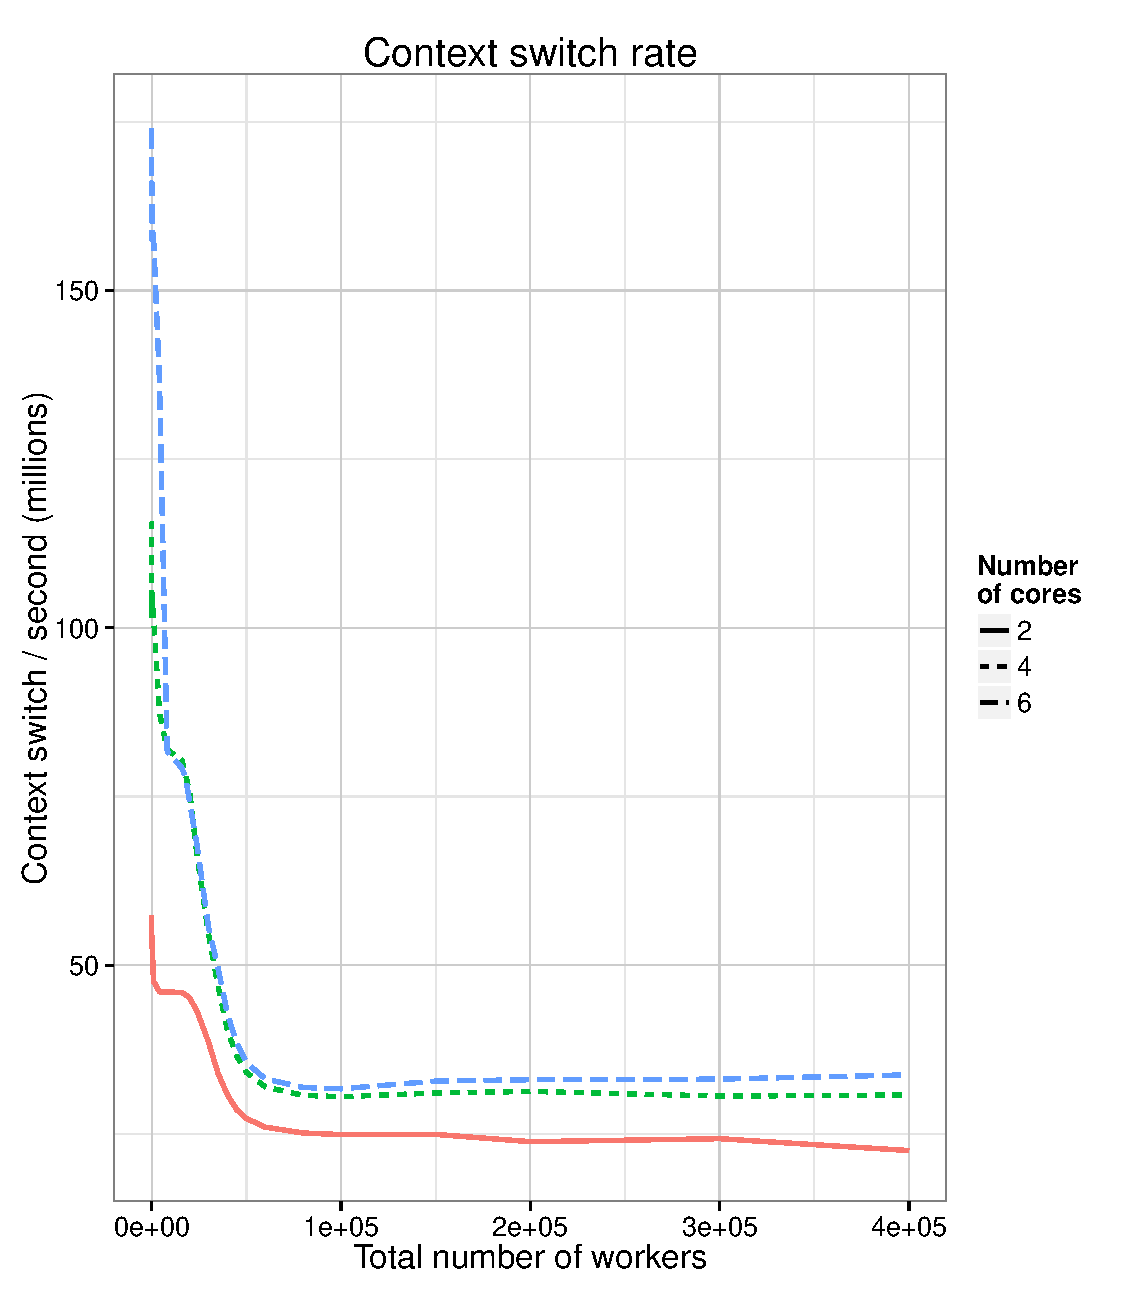
\includegraphics[width=0.5\textwidth]{figs/context_switch_bw.pdf}
    \end{center}
    \caption{Context switch rate with prefetching. Once the total
        size of contexts sufficiently exceeds last-level cache, most
    prefetches go to main memory and the rate becomes limited to the
    off-chip bandwidth.}
    \label{fig:context-switch-time}
\end{figure}

\TODO{Summary of what to write please expand: Reference above plots. Bandwidth of single socket is
    270Mcacheline/s. Each context is 4 cachelines: 1 for worker struct
    and 3 stack cachelines. We must read and write every context, so 8
    cacheline transfers per context switch. This asymptotically
    approaches 33.75Mcontexts/s as you increase the number of contexts
    (fewer and fewer in L3). Note that only 4+ cores reaches full rate
    because these westmere chips are balanced to not achieve full off-chip bandwidth until 4
    cores--bdmyers}

\TODO{Yield test results:  latency \& bandwidth.  Discussion of implications of zillions of contexts on robustness of latency tolerance preshadowing ~\ref{sec:scaling}}

\subsection{Application Results}
To evaluate \Grappa's performance with respect to the XMT, we ran each
of our three benchmarks on up to 16 nodes of each machine. \Grappa used
6 cores per node, with the best parameters chosen for each point. In
some cases, the XMT could not run the benchmark with 2 nodes, so the
point is omitted. \TODO{rewrite this!}
\subsubsection{Unbalanced Tree Search}\TODO{rewrite with new results}
%% UTS: performance comparison
\begin{figure}[ht]
    \begin{center}
      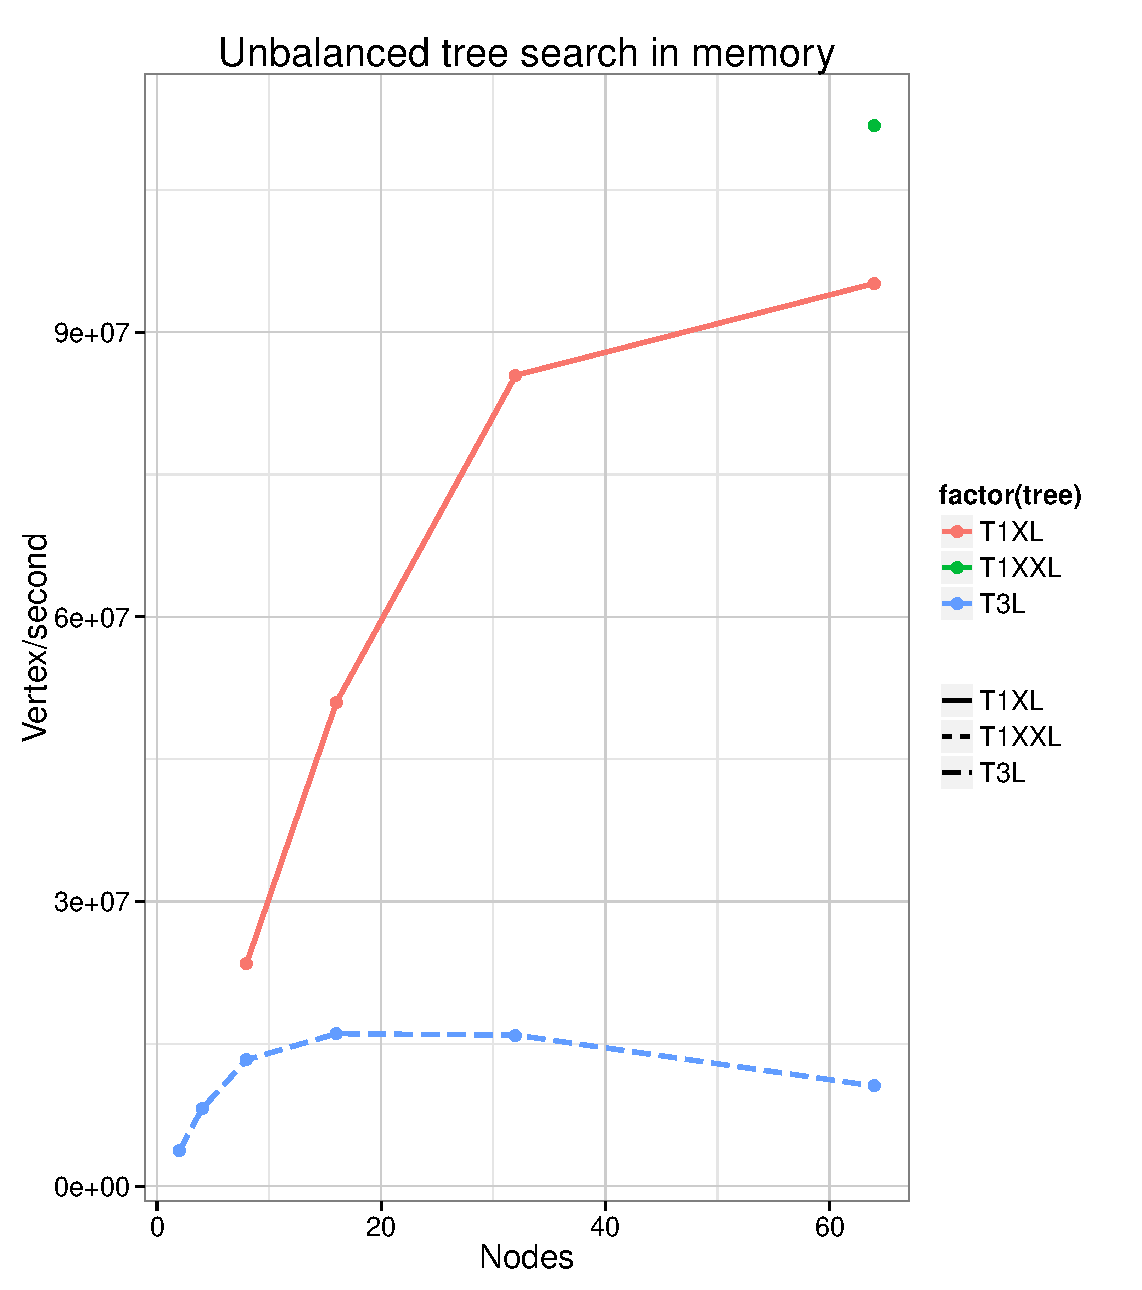
\includegraphics[width=0.5\textwidth]{figs/uts_scale.pdf}
    \end{center}
    \caption{Performance of in-memory unbalanced tree search.}
    \label{fig:uts_compare}
\end{figure}

We ran UTS-mem with a geometric 100M-vertex tree
(T1L). Figure~\ref{fig:uts_compare} shows the performance in terms of
number of vertices visited per second versus number of compute
nodes. \Grappa is 3.2 times faster than the XMT at 16 nodes.  As we will show later, the performance advantage \Grappa has over XMT increases as more nodes are added.  The main reason \Grappa performs better is the software-based delegate synchronization obviates the need for the retry-based synchronization that XMT uses.

\subsubsection{Breadth First Search}\TODO{rewrite with new results}
\begin{figure}[tH]
\begin{center}
  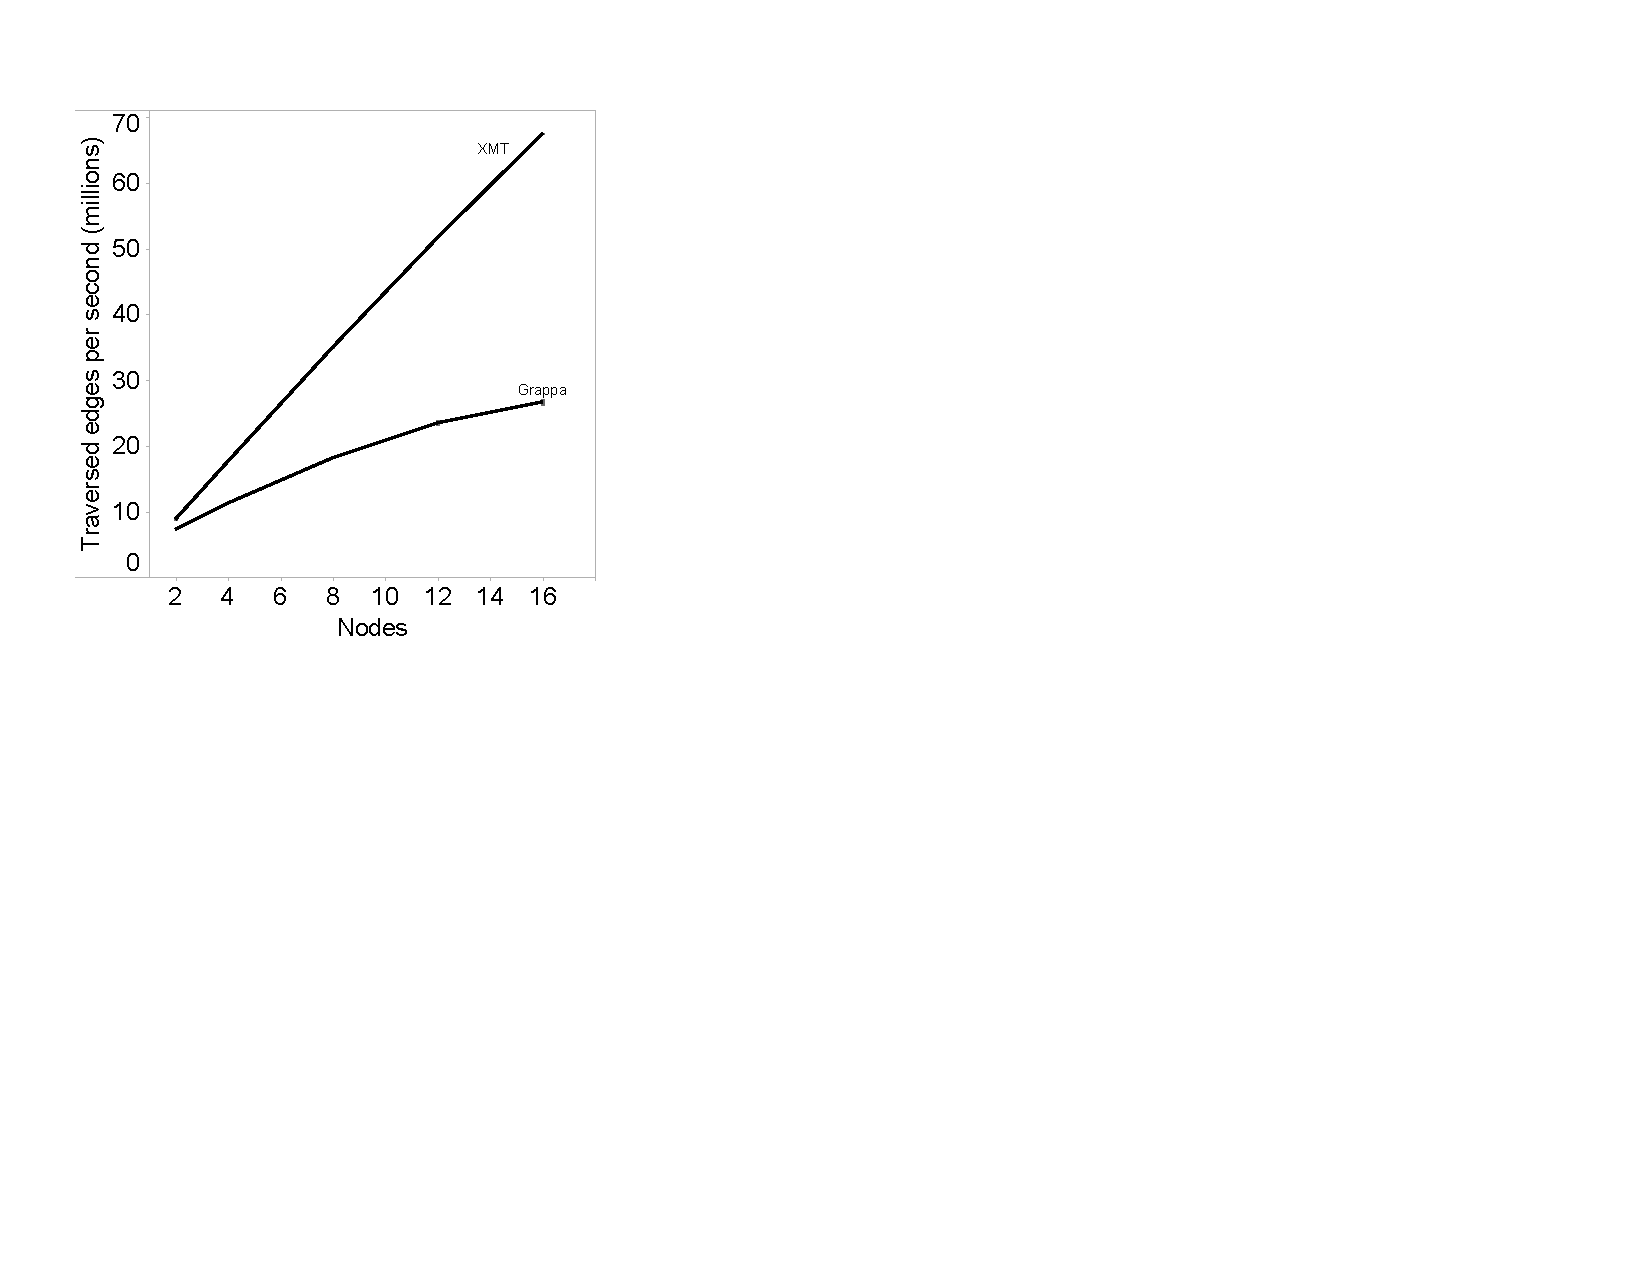
\includegraphics[width=0.95\columnwidth]{figs/bfs_performance}
\begin{minipage}{0.95\columnwidth}
  \caption{\label{fig:bfs-performance} BFS performance}
\end{minipage}
\vspace{-3ex}
\end{center}
\end{figure}

We ran BFS on a synthetic Kronecker graph with $2^{25}$ vertices and
$2^{29}$ edges (25 GB of data). Figure~\ref{fig:bfs-performance} shows
our performance in terms of graph edges traversed per second. The XMT
is 2.5 times faster than \Grappa at 16 nodes.  Performance does scale at a constant rate for \Grappa, suggesting that adding more nodes will increase performance.

\subsubsection{Approximate Betweenness Centrality}\TODO{rewrite with new results}
\begin{figure}[tH]
\begin{center}
  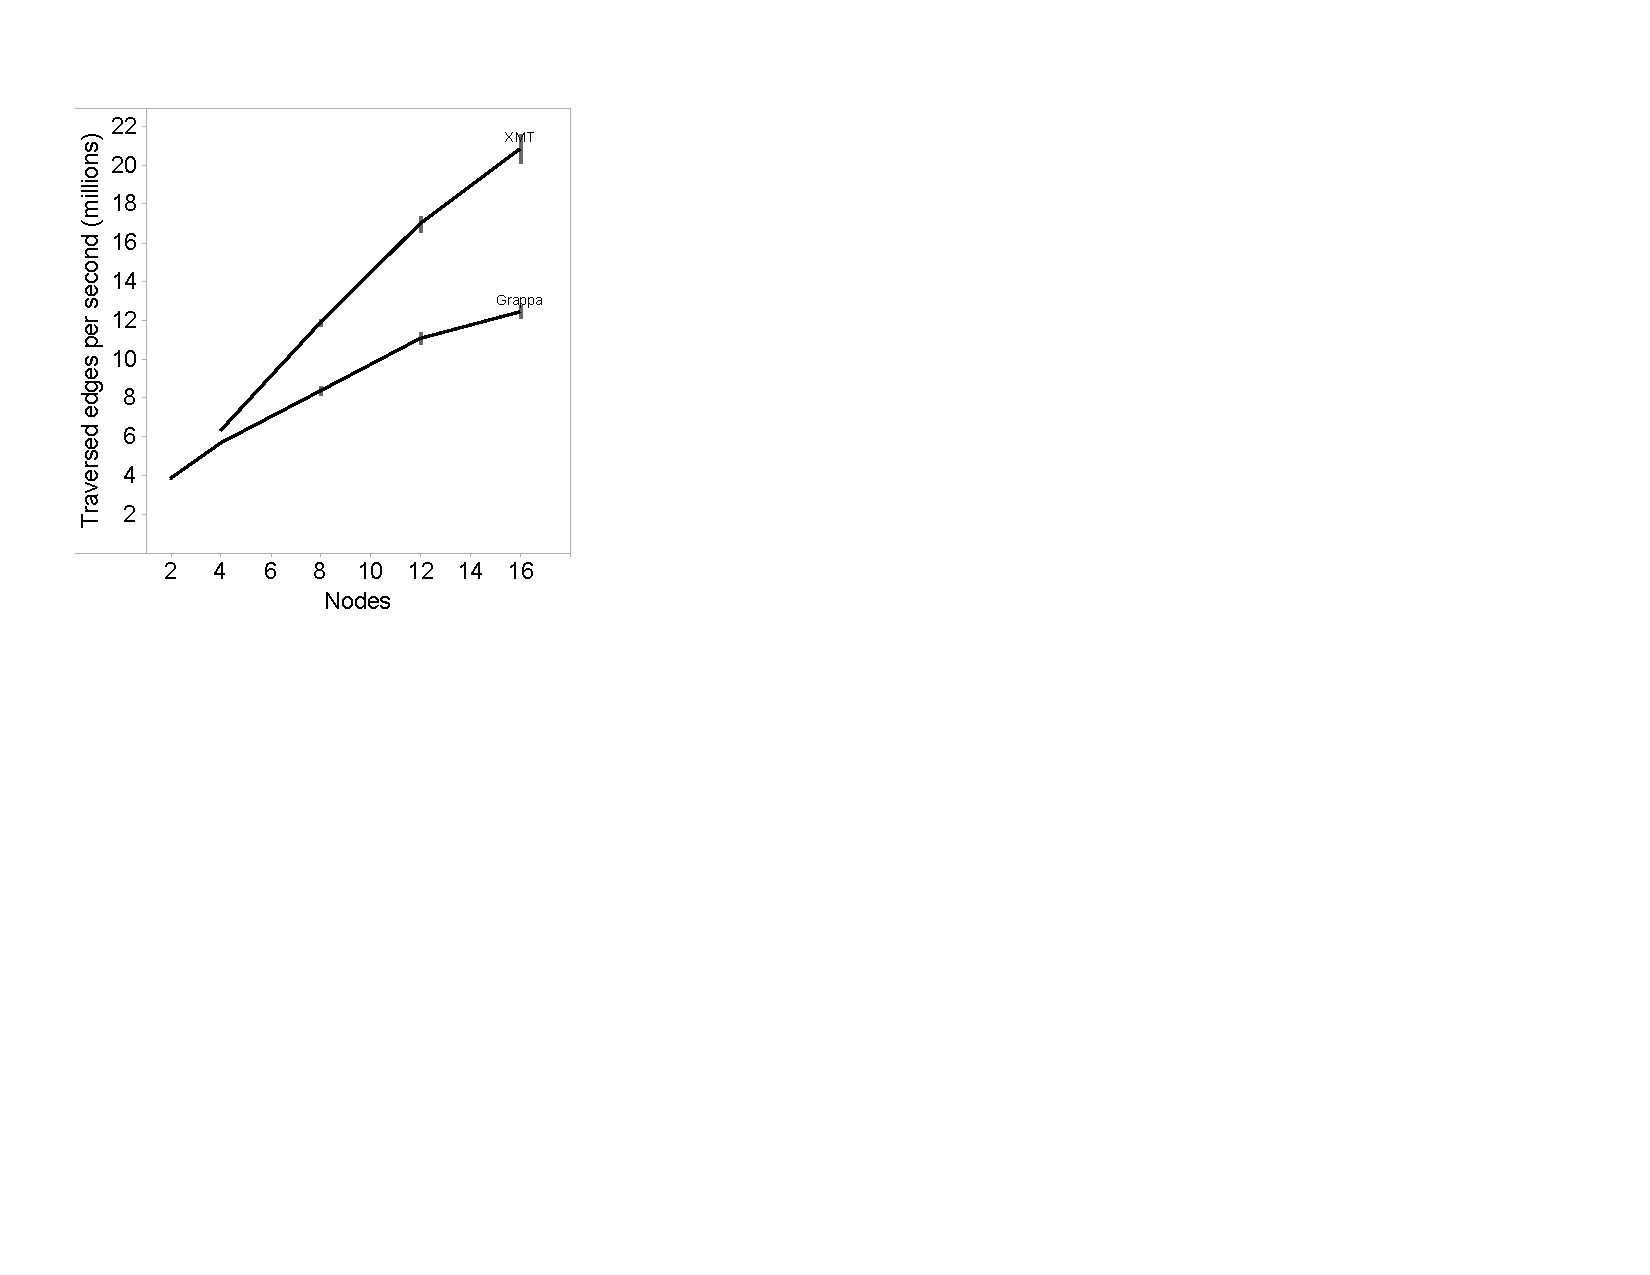
\includegraphics[width=0.95\columnwidth]{figs/centrality_performance}
\begin{minipage}{0.95\columnwidth}
  \caption{\label{fig:centrality-performance} Centrality performance}
\end{minipage}
\vspace{-3ex}
\end{center}
\end{figure}

We ran Betweenness Centrality on the same scale 25 Kronecker graph as
we did for BFS. Figure~\ref{fig:centrality-performance} shows our
performance in terms of graph edges traversed per second. At 16 XMT
processors/cluster nodes, the XMT is 1.75 times faster than \Grappa.

% Got rid of this discussion of UTS by itself, tried to work the highlights in below
%\paragraph{UTS-Mem}
%We ran UTS-Mem on \Grappa and the XMT with a geometric 1.6B-vertex tree
%(T1XL) and a geometric 4.2B-vertex tree (T1XXL), using up to 128
%nodes---the maximum we had available for each. \Grappa results are for 5 cores per node. \Grappa with 20 machines is faster than the entire XMT of 128 processors.

%\Grappa achieves \checkme{188Mvert/s} with 128 nodes and the XMT
%achieves only 50Mvert/s, plateauing at 60 nodes. Beyond 90 nodes, \Grappa adds 1.4 Mvert/s/node.
%The XMT scales at 850 Kvert/s/node, until it plateaus. \Grappa keeps
%scaling up through 128 nodes, although scaling
%declines because of the unscalability of our aggregation mechanism as
%number of network endpoints increases. 
%
%Despite our efforts to tune the UTS implementation specific to the 
%XMT, performance does not scale well with increasing processor count,
%flattening out around 60 processors.  When we increase the size of
%the tree from 100M to 4.2B, we find that performance does not improve,
%suggesting that performance is not limited by task parallelism.
%Cray's performance tools show an increasing number of memory
%retry operations for failed synchronization operations generated by
%the runtime, which create network contention.
%
To determine how \Grappa's performance scales compared to the performance of the entire XMT, we ran a set of experiments up to all 128 XMT processors and 128 cluster nodes. For the XMT, the number of allowed processors was varied up to the entire machine, with some minor tuning of stream parameters needed to get optimal performance. For \Grappa, parameters such as cores per node, aggregator timeouts, and parallel threshold were tuned to get the best performance for each node count. All of the benchmarks continue to improve out to 128 nodes for \Grappa. UTS continues to fare better than the XMT with large node counts, with the XMT appearing to plateau at 60 processors due to contention from synchronization retries, while \Grappa handles this by suspending tasks until messages return. For BFS and Centrality, the XMT scales approximately a constant factor better than \Grappa. We attribute this to a limitation in the current aggregator design and network stack that \Grappa uses.  This limits the practical number of cores we can use to 6 per node (adding more cores per node \emph{decreases} performance).  Ironically, this limitation makes \Grappa applications compute-bound instead of network-bound.  Work is ongoing to rework the Infiniband driver stack and aggregation interface to remove this limitation and improve aggregation addressing using local routing.

\begin{figure}[ht]
    \begin{center}
      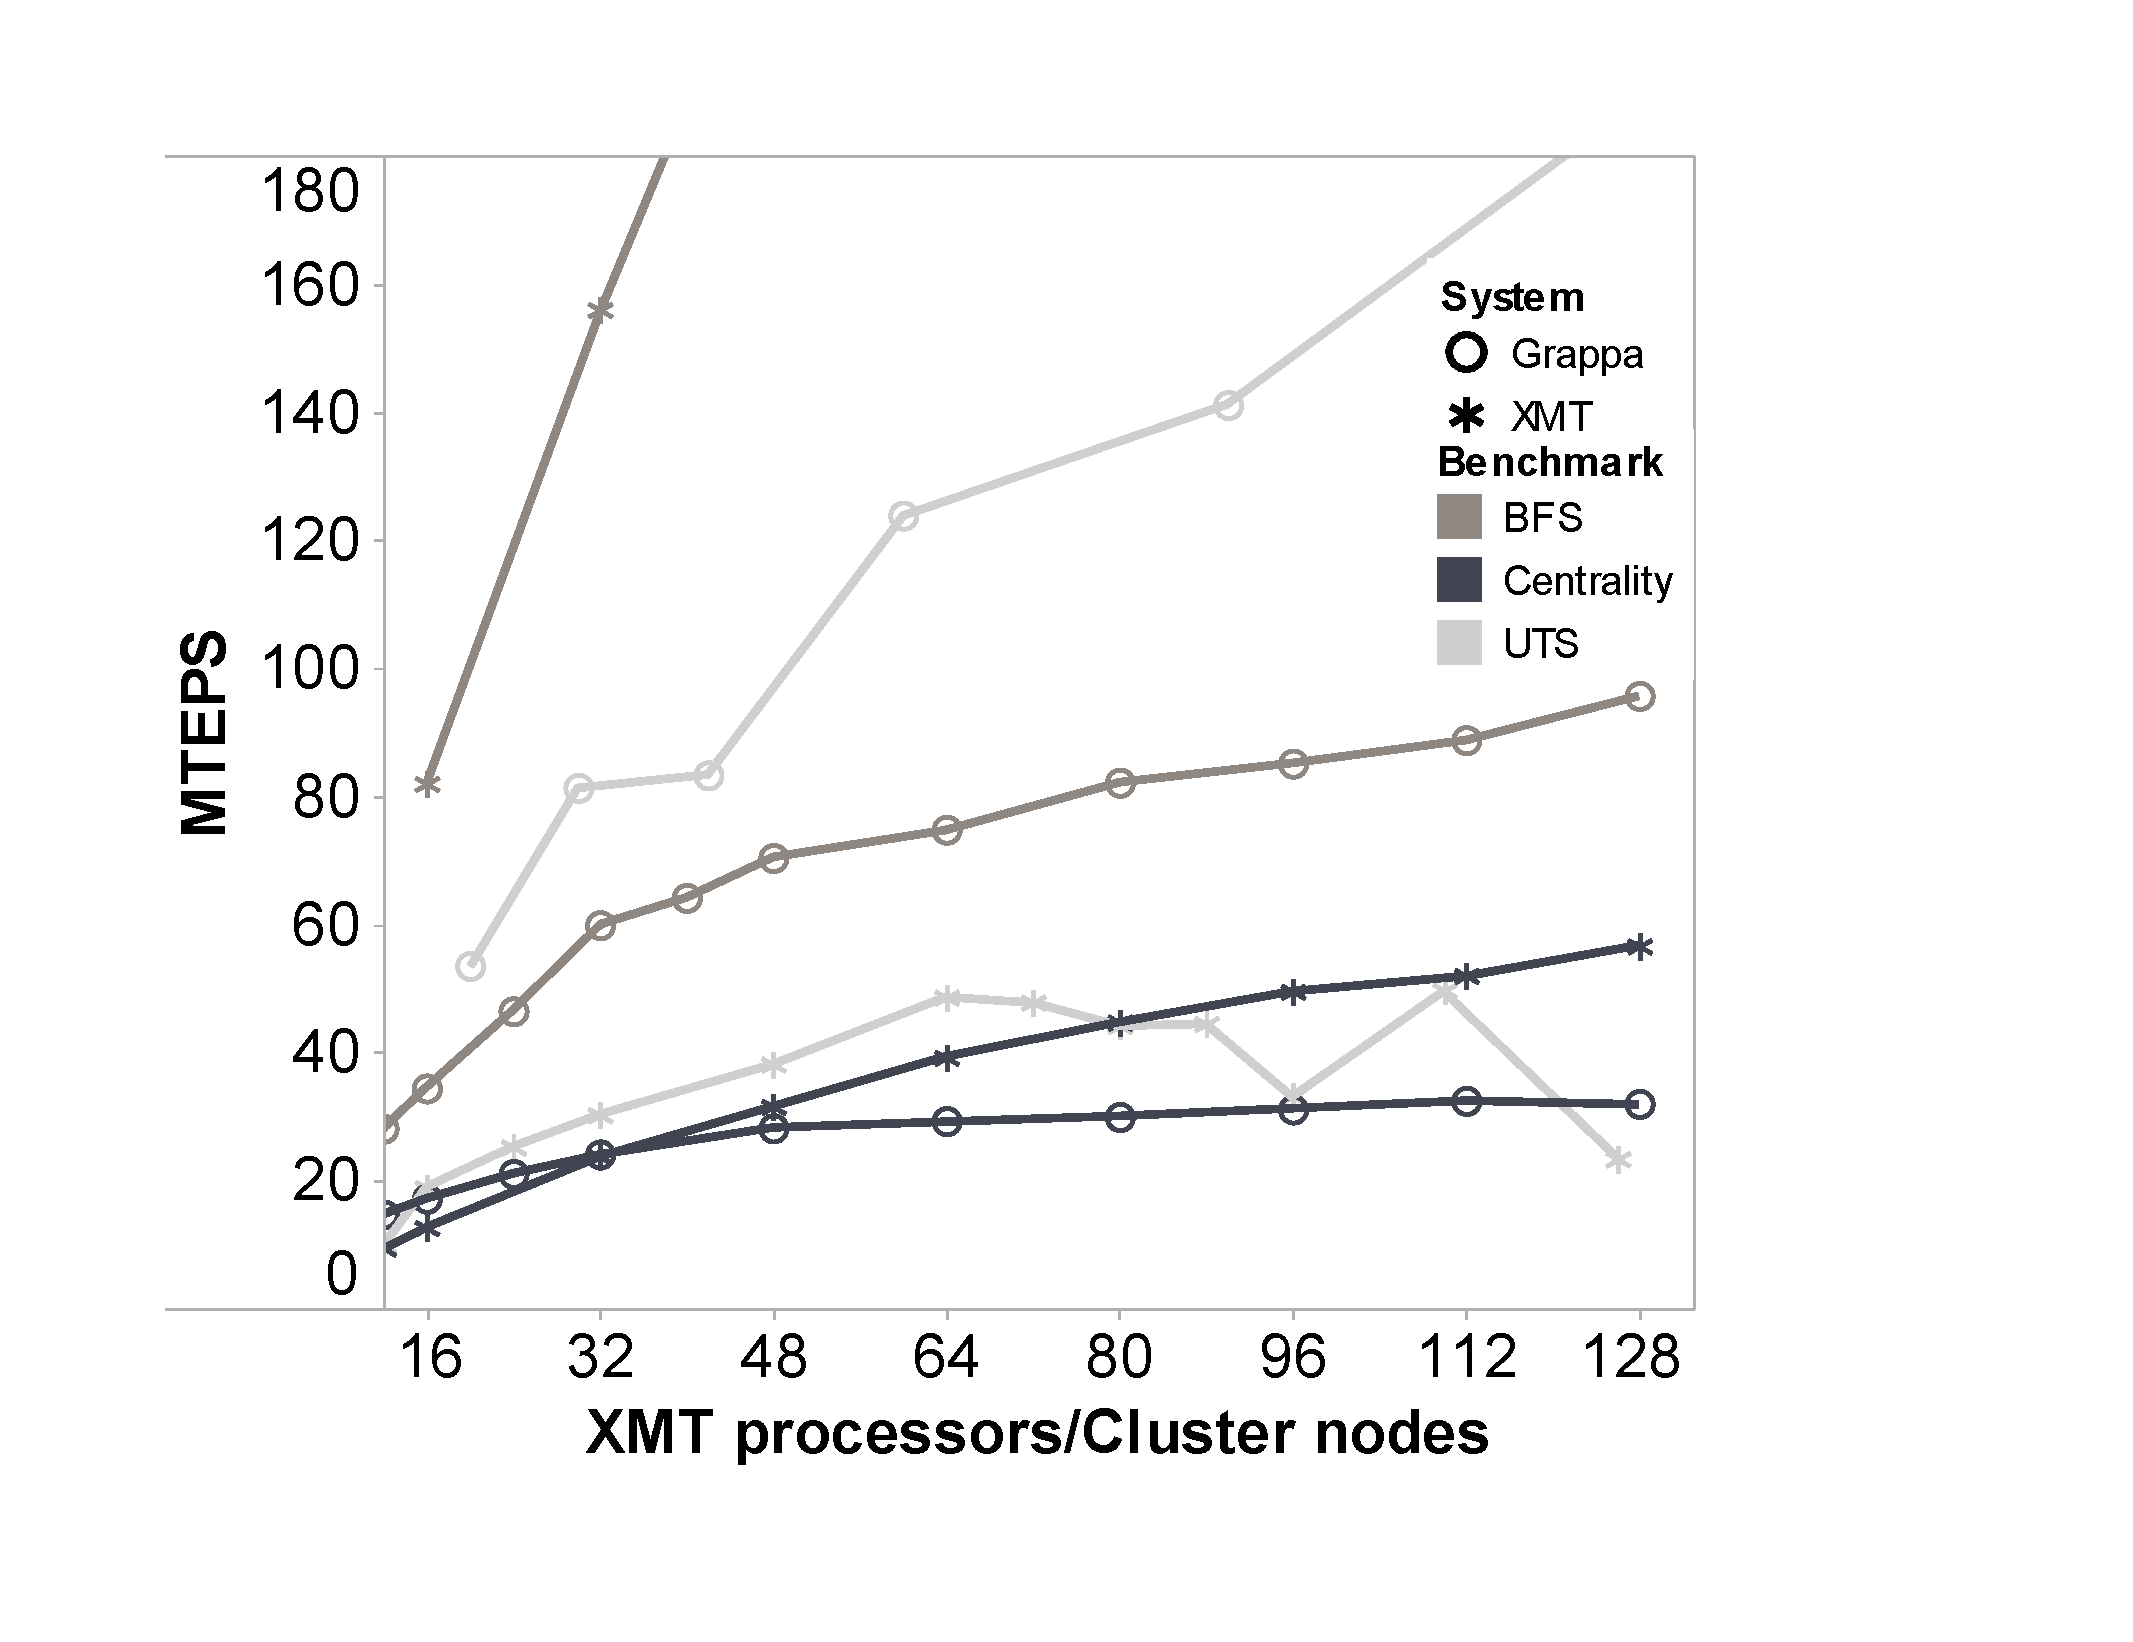
\includegraphics[width=0.5\textwidth]{figs/scaling_cropped.pdf}
    \end{center}
    \caption{Scaling number of nodes: \Grappa continues to perform significantly better than XMT for UTS but scales a constant factor slower than XMT for BFS (4x slower) and Centrality (2x slower). }
    \label{fig:uts_threshold}
\end{figure}

\subsection{Scaling}\label{sec:scaling} \TODO{rewrite with new results}

\subsubsection{Network Aggregation Performance and Robustness}

\begin{figure}[htb]
\begin{center}
  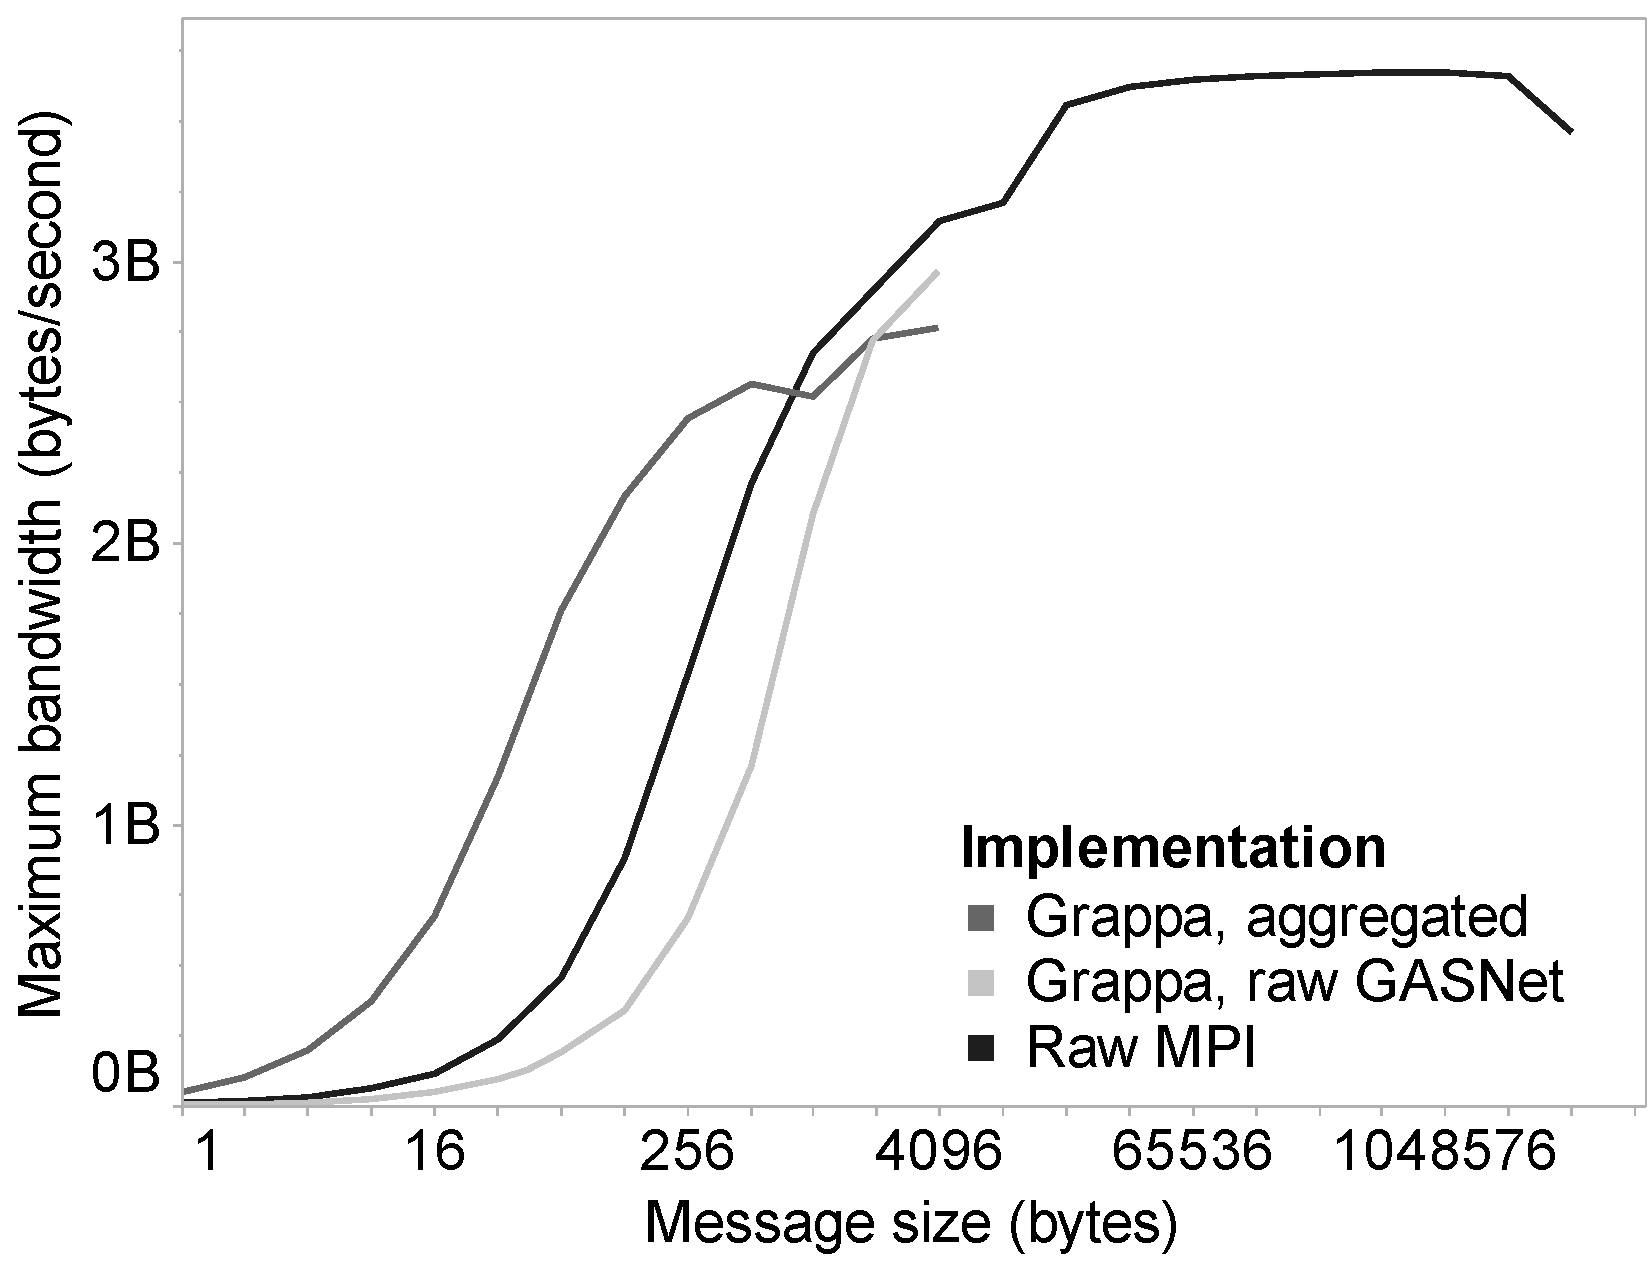
\includegraphics[width=0.95\columnwidth]{figs/aggregator_ping}
\begin{minipage}{0.95\columnwidth}
  \caption{\label{fig:aggregator-ping} Bandwidth versus message size
    unidirectional ping test for \Grappa with aggregation, \Grappa with
    raw GASNet messages, and MPI. Aggregation provides an 11x
    bandwidth benefit at our common operating point.}
\end{minipage}
\vspace{-3ex}
\end{center}
\end{figure}

To evaluate the benefits of network aggregation, we ran two experiments.
First, we ran a simple unidirectional ping test to see the maximum
benefit the aggregator can provide in terms of improved network
efficiency. Second, we ran BFS with the aggregator disabled in order to
measure its benefit on an application.

To implement the ping test, we wrote a simple \Grappa application where
the cores of one node send messages as fast as possible to the cores
of another node. We vary the size of the payload up the maximum
payload size supported by the aggregator (nearly 4KB). Each core has a
single task sending to a single destination, so this is a best case
scenario for the aggregator. To see the benefit of the aggregator, we
added a bypass that lets us send messages directly through GASNet. We
also compare against the OSU \texttt{osu\_mbw\_mr} benchmark
\cite{osu:mpi}  compiled against OpenMPI 1.5.3; this
benchmark has the same pattern of communication but doesn't have the
overhead of \Grappa's context switching.

The results are shown in Figure~\ref{fig:aggregator-ping}. There are
two key observations.

First, small message performance against the existing libraries is, as expected, poor. The MPI application test shows us that peak per node
bandwidth supported by our infiniband card is 3.4GB/s. This is
achievable only with large messages; we must send 16KB packets to get
within 5 percent of peak bandwidth. But in our benchmarks, we saw
average message between 32 and 64 bytes. At 32 bytes, the MPI test is
using less than 7 percent of its peak bandwidth. \Grappa sending
messages directly through GASNet uses less than 3 percent of the peak
bandwidth.

Second, aggregation has the potential to improve this situation by an
order of magnitude. With aggregation, \Grappa is able to send 32-byte
messages over 12 times faster than using GASNet directly. This is a
more respectable 32 percent of peak bandwidth. Due to expedient design
decisions, \Grappa's aggregator limits its aggregation to 4KB; this
limits its peak achievable bandwidth to 75 percent of the actual
peak.

This comparison is the best possible case for the aggregator. In
order to verify that the aggregator still has value on actual
applications at scale, we ran a small (100M node tree) UTS-Mem
with the aggregator disabled, on 16 nodes.
Figure~\ref{fig:no-aggregation-uts}. At this configuration, the aggregator
improves our application performance by 10x. 

\begin{figure}[htb]
\begin{center}
  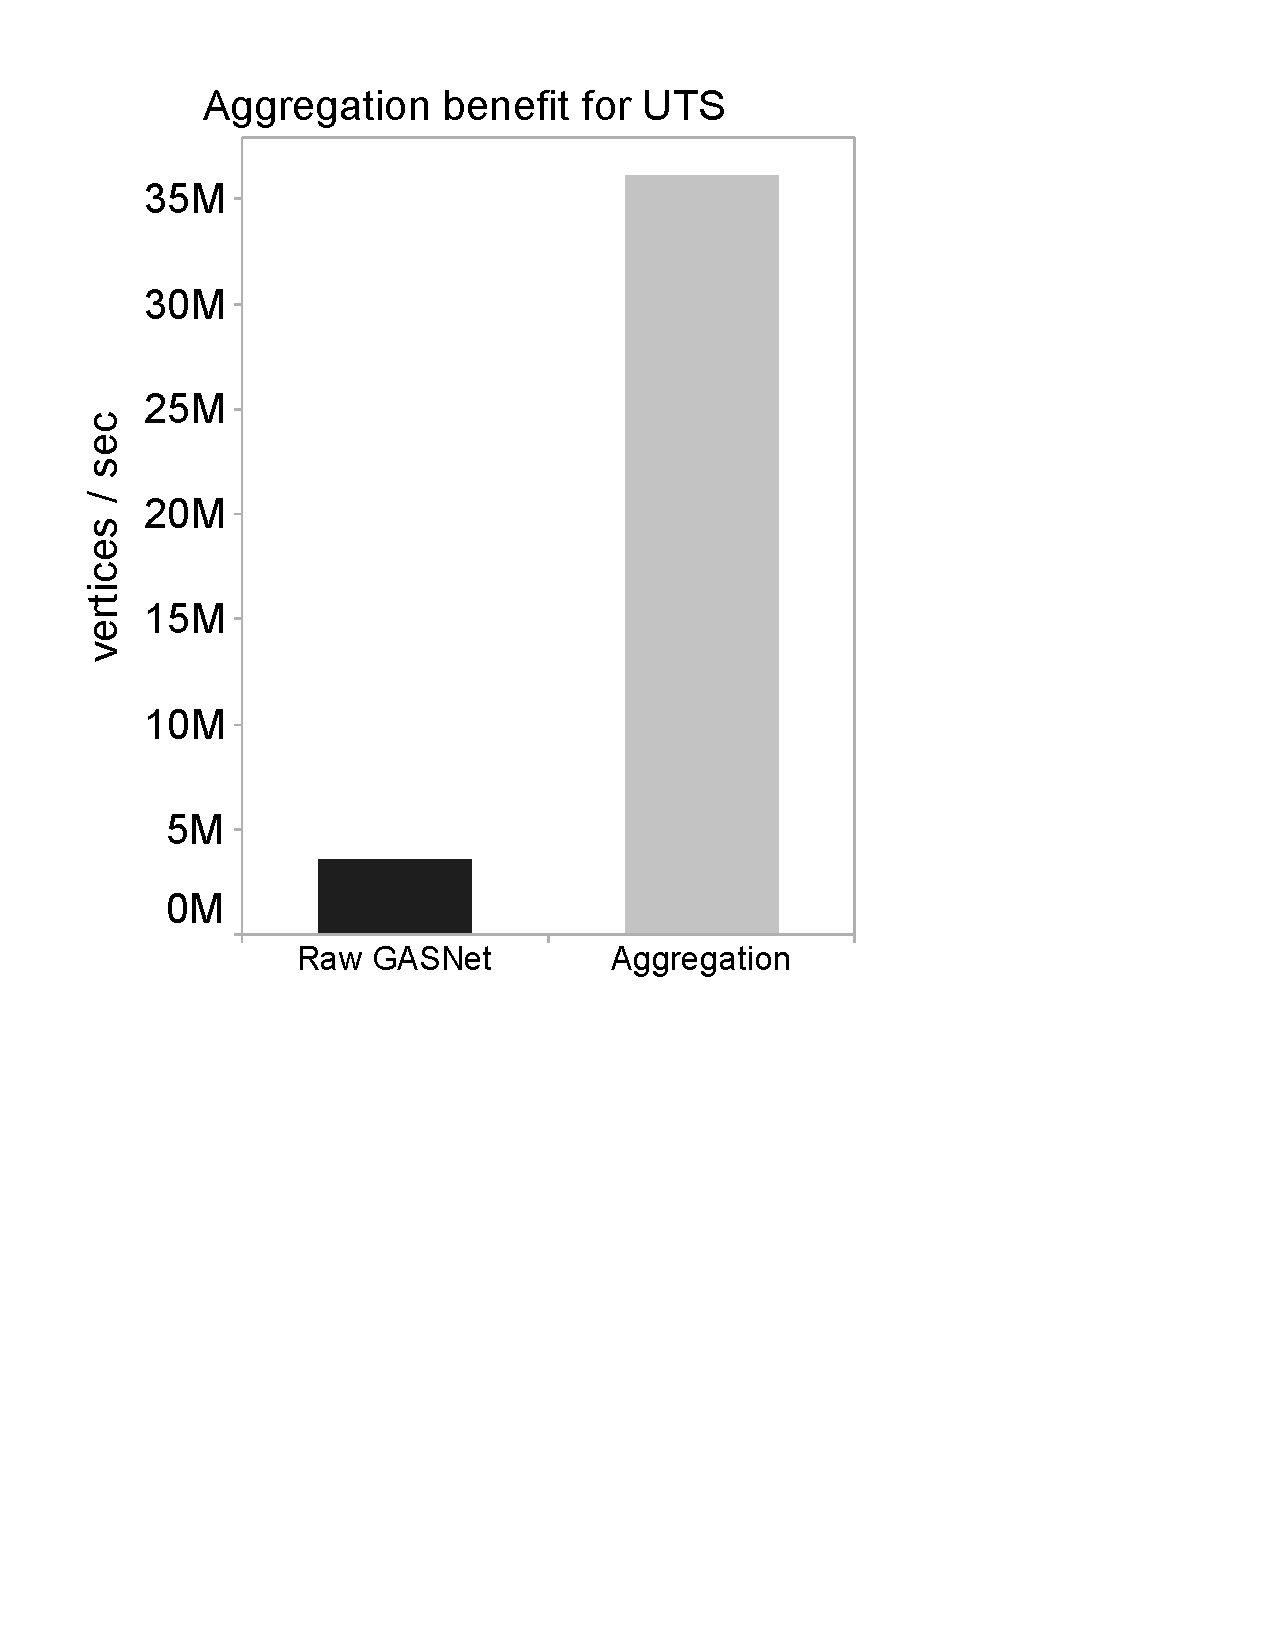
\includegraphics[width=0.95\columnwidth]{figs/no_aggregation_uts.pdf}
\begin{minipage}{0.95\columnwidth}
  \caption{\label{fig:no-aggregation-uts} Performance of UTS on 16
      nodes with and without \Grappa's aggregation.}
\end{minipage}
\vspace{-3ex}
\end{center}
\end{figure}

\subsection{Scaling}
% Got rid of this discussion of UTS by itself, tried to work the highlights in below
%\paragraph{UTS-Mem}
%We ran UTS-Mem on \Grappa and the XMT with a geometric 1.6B-vertex tree
%(T1XL) and a geometric 4.2B-vertex tree (T1XXL), using up to 128
%nodes---the maximum we had available for each. \Grappa results are for 5 cores per node. \Grappa with 20 machines is faster than the entire XMT of 128 processors.
%\Grappa achieves \checkme{188Mvert/s} with 128 nodes and the XMT
%achieves only 50Mvert/s, plateauing at 60 nodes. Beyond 90 nodes, \Grappa adds 1.4 Mvert/s/node.
%The XMT scales at 850 Kvert/s/node, until it plateaus. \Grappa keeps
%scaling up through 128 nodes, although scaling
%declines because of the unscalability of our aggregation mechanism as
%number of network endpoints increases. 
%
%Despite our efforts to tune the UTS implementation specific to the 
%XMT, performance does not scale well with increasing processor count,
%flattening out around 60 processors.  When we increase the size of
%the tree from 100M to 4.2B, we find that performance does not improve,
%suggesting that performance is not limited by task parallelism.
%Cray's performance tools show an increasing number of memory
%retry operations for failed synchronization operations generated by
%the runtime, which create network contention.
%
To determine how \Grappa's performance scales compared to the performance of the entire XMT, we ran a set of experiments up to all 128 XMT processors and 128 cluster nodes. For the XMT, the number of allowed processors was varied up to the entire machine, with some minor tuning of stream parameters needed to get optimal performance. For \Grappa, parameters such as cores per node, aggregator timeouts, and parallel threshold were tuned to get the best performance for each node count. All of the benchmarks continue to improve out to 128 nodes for \Grappa. UTS continues to fare better than the XMT with large node counts, with the XMT appearing to plateau at 60 processors due to contention from synchronization retries, while \Grappa handles this by suspending tasks until messages return. For BFS and Centrality, the XMT scales approximately a constant factor better than \Grappa. We attribute this to a limitation in the current aggregator design and network stack that \Grappa uses.  This limits the practical number of cores we can use to 6 per node (adding more cores per node \emph{decreases\/} performance).  Ironically, this limitation makes \Grappa applications compute-bound instead of network-bound.  Work is ongoing to rework the Infiniband driver stack and aggregation interface to remove this limitation and improve aggregation addressing using local routing.

\begin{figure}[ht]
    \begin{center}
      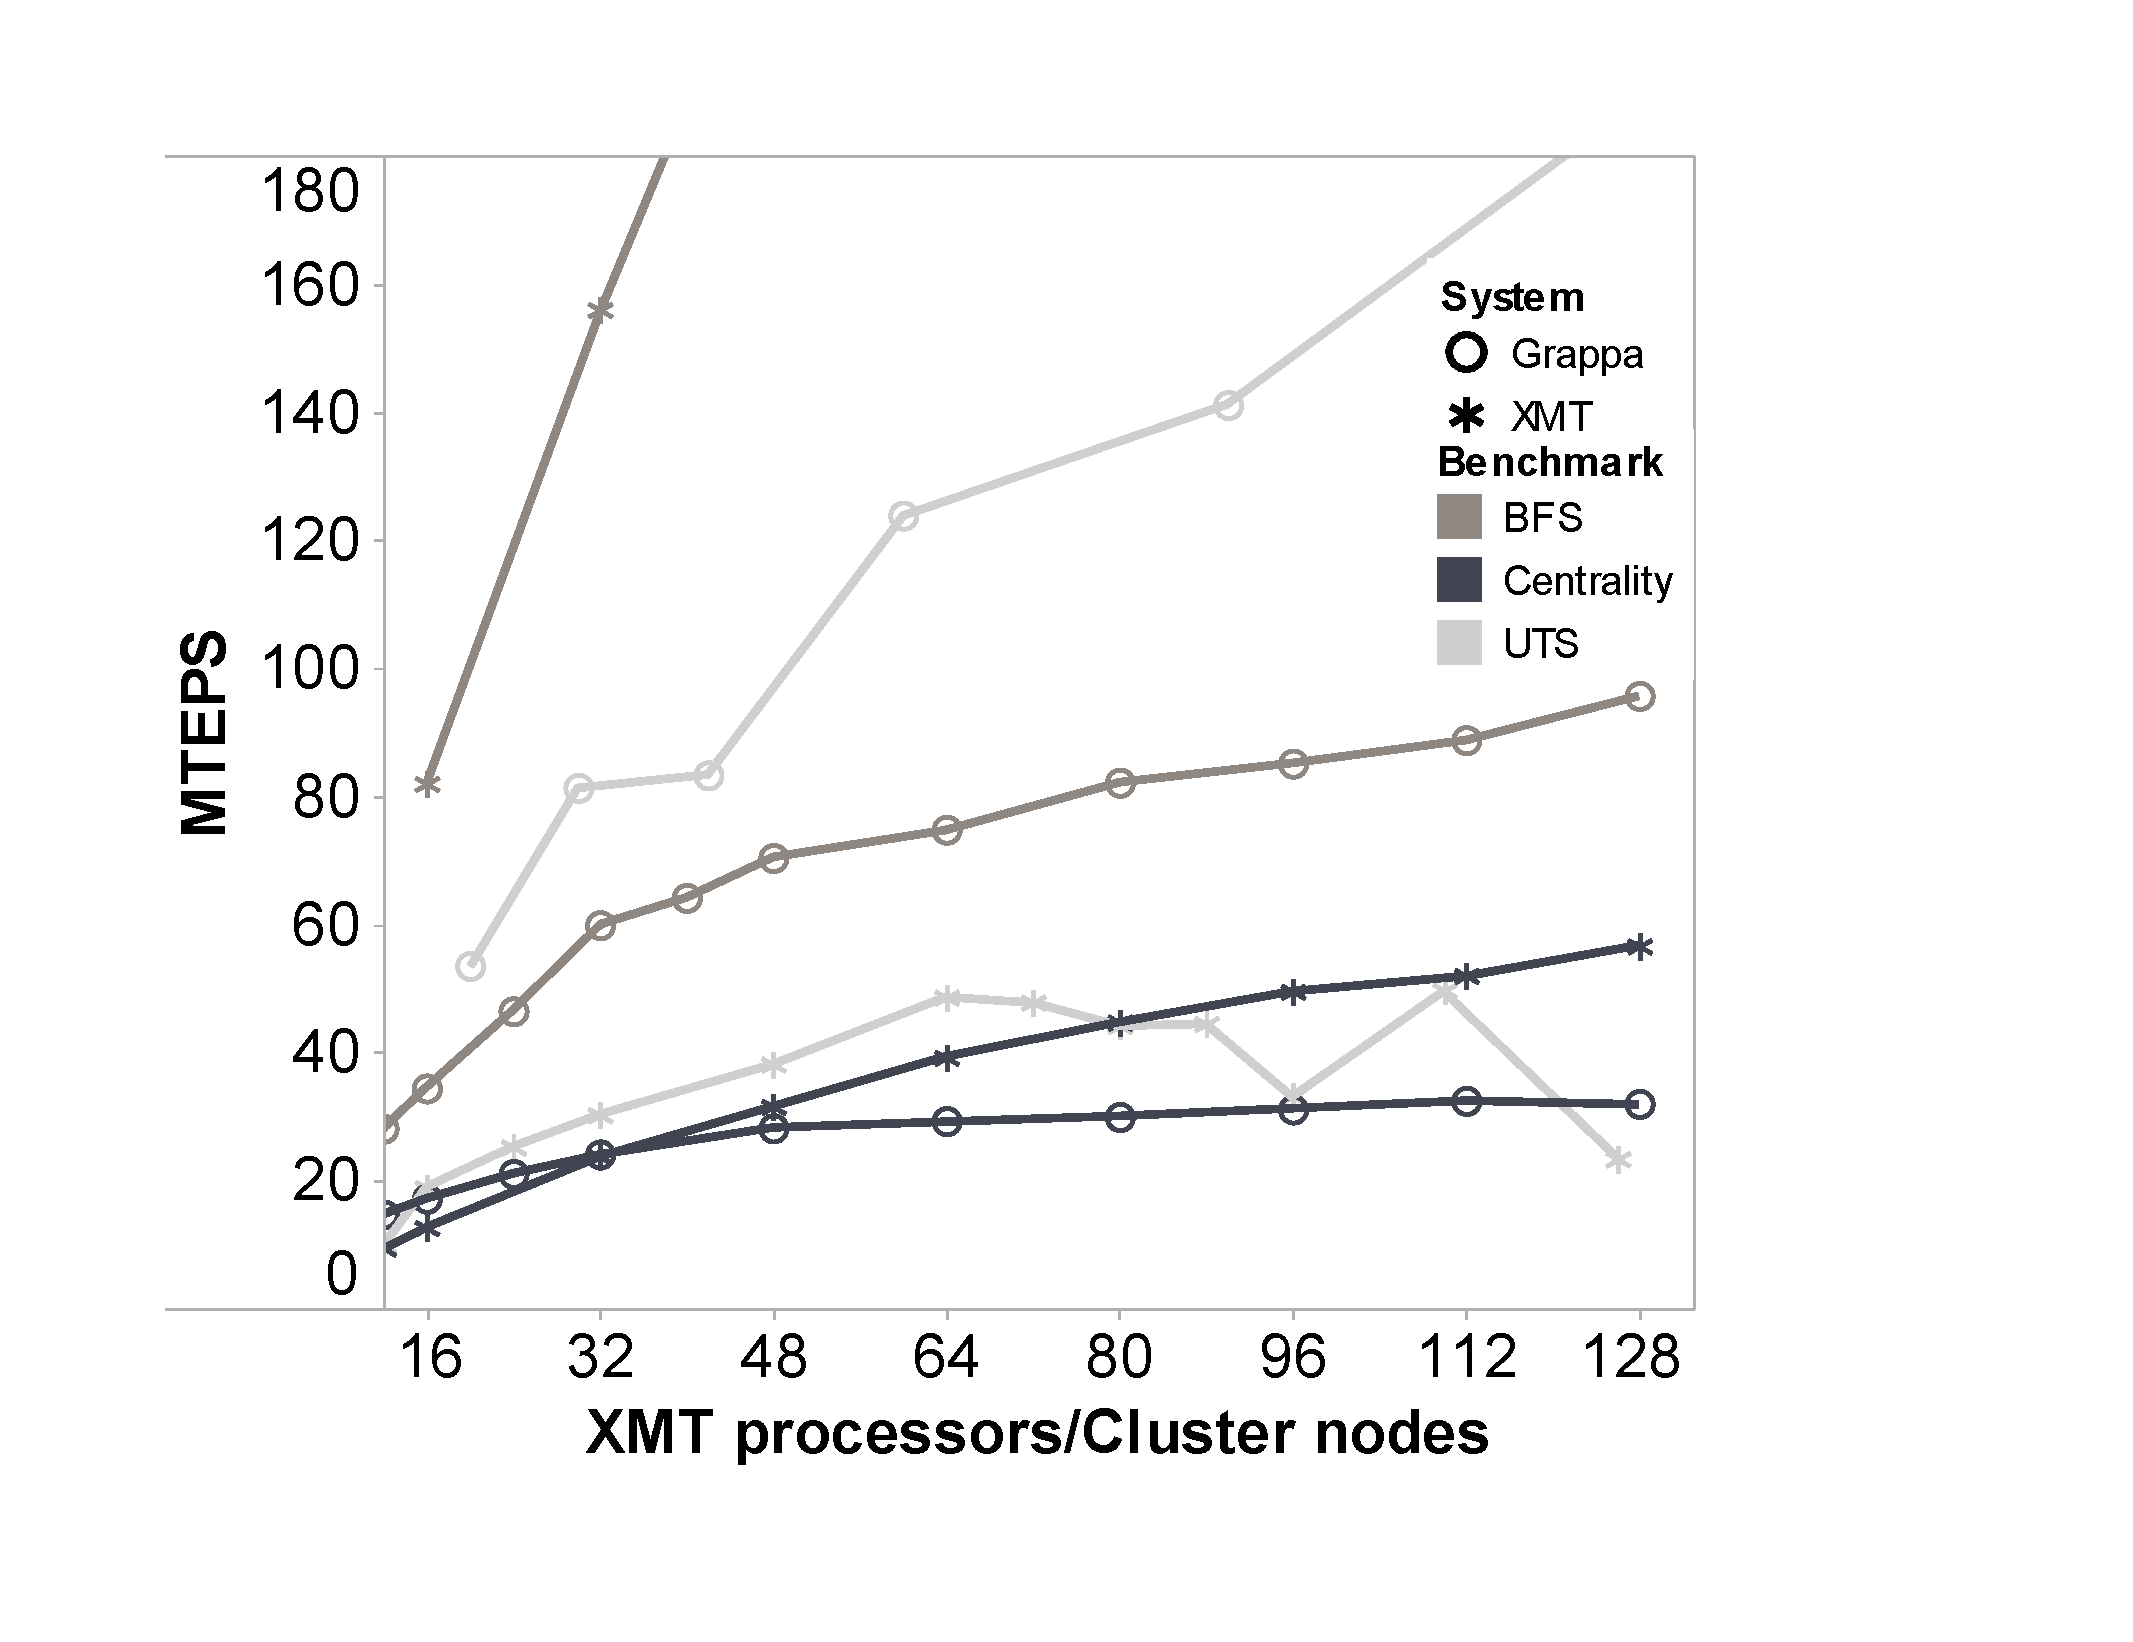
\includegraphics[width=0.5\textwidth]{figs/scaling_cropped.pdf}
    \end{center}
    \caption{Scaling number of nodes: \Grappa continues to perform significantly better than XMT for UTS but scales a constant factor slower than XMT for BFS (4x slower) and Centrality (2x slower). }
    \label{fig:uts_threshold}
\end{figure}


\subsection{Sensitivity}

\paragraph{Aggregator timeout}

\begin{figure}[htb]
\begin{center}
  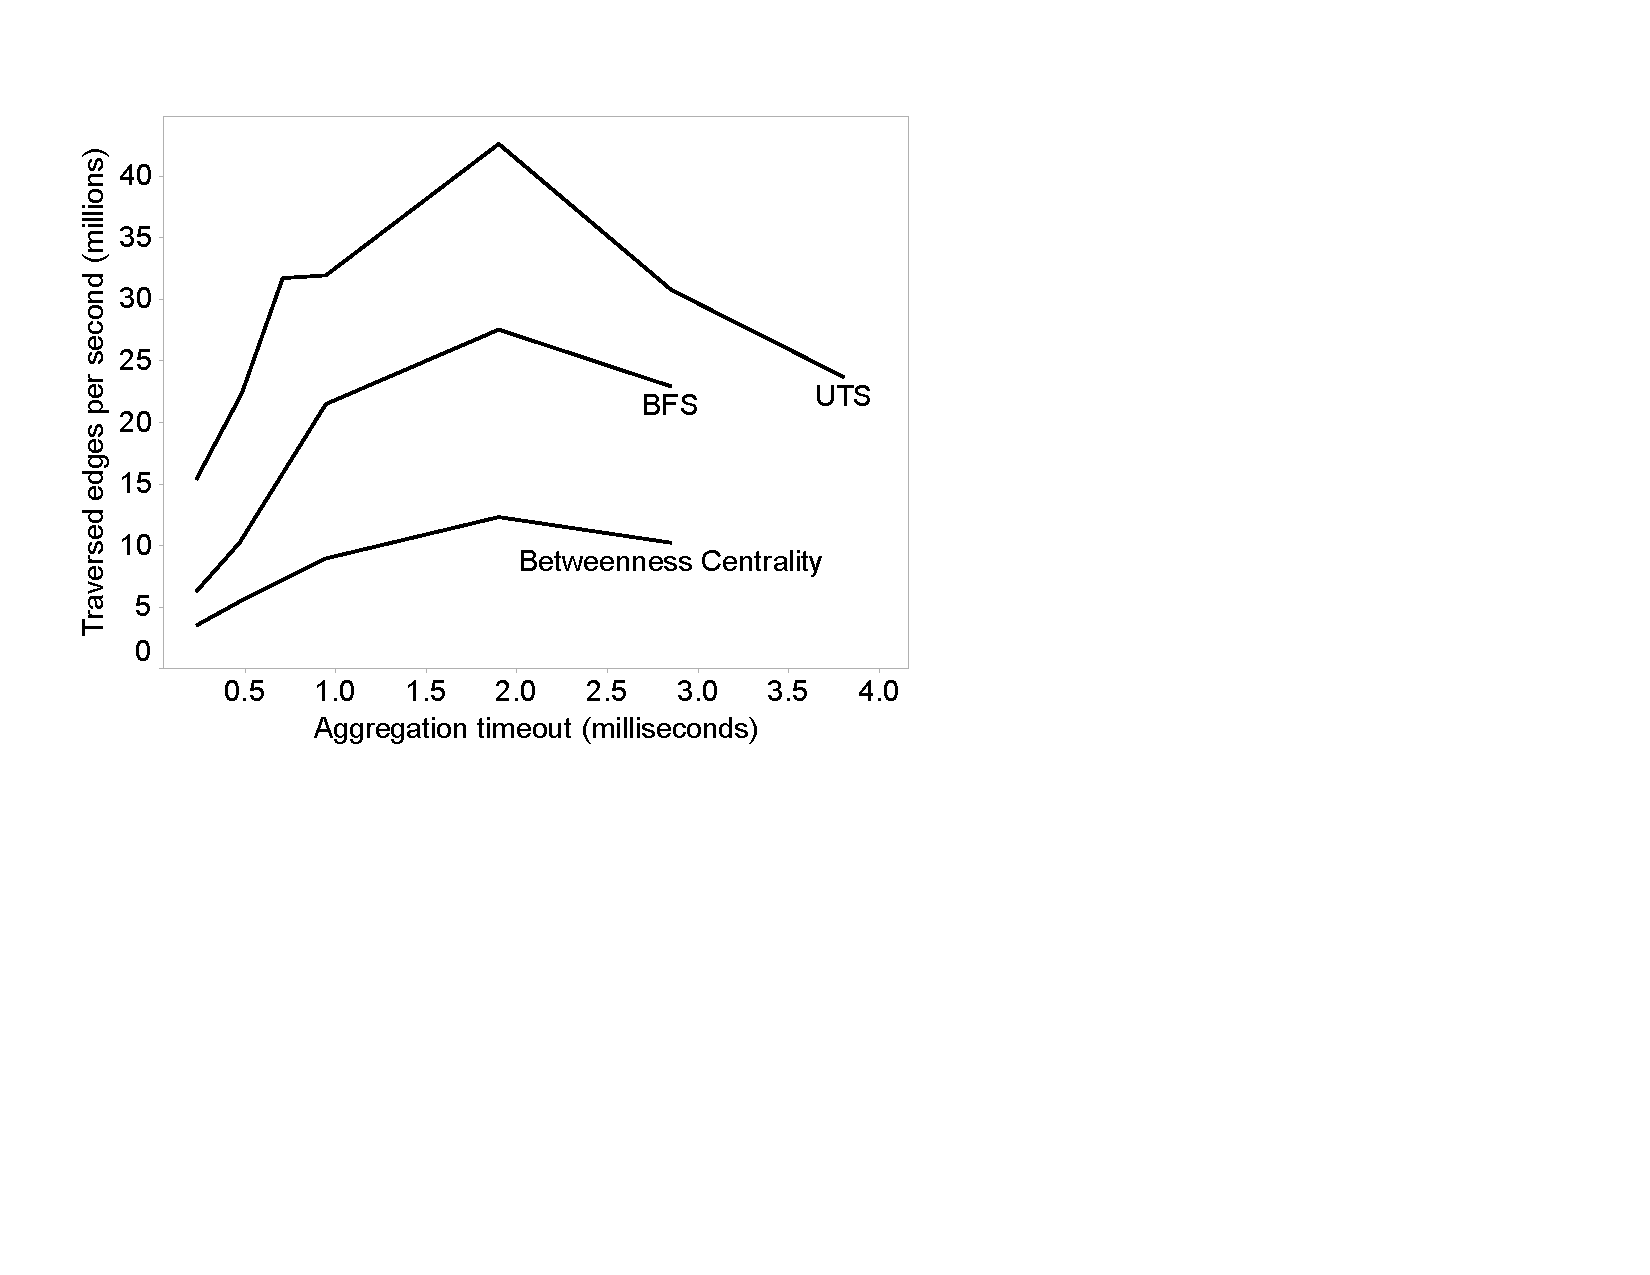
\includegraphics[width=0.95\columnwidth]{figs/flushticks_sweep}
\begin{minipage}{0.95\columnwidth}
  \caption{\label{fig:bfs-sweep-flushticks} Sensitivity to aggregation delay}
\end{minipage}
\vspace{-3ex}
\end{center}
\end{figure}


One of the key parameters of the aggregator is the message
timeout. All messages that are queued must eventually be sent in order
to ensure progress. In the best case, we are able to aggregate enough
messages to fill an aggregation buffer and cause it to be sent, but as
we scale up, the average rate of messages heading to a common
destination decreases, and this gets harder. To bound the problem, the
aggregator includes a timeout. Any packet waiting this long is sent
the next time the communications layer is serviced.

Figure~\ref{fig:bfs-sweep-flushticks} shows a sweep of this parameter
for UTS, BFS, and Betweenness Centrality on 16 nodes, using the
datasets described previously. The maximum number of workers is fixed
at 2048. All the benchmarks show a performance peak with a 2
millisecond timeout; at this point we are delaying long enough to
aggregate the largest packets we can; setting the parameter higher
causes tasks to wait longer for responses, but few new requests are
being generated.


\begin{figure}[htb]
\begin{center}
  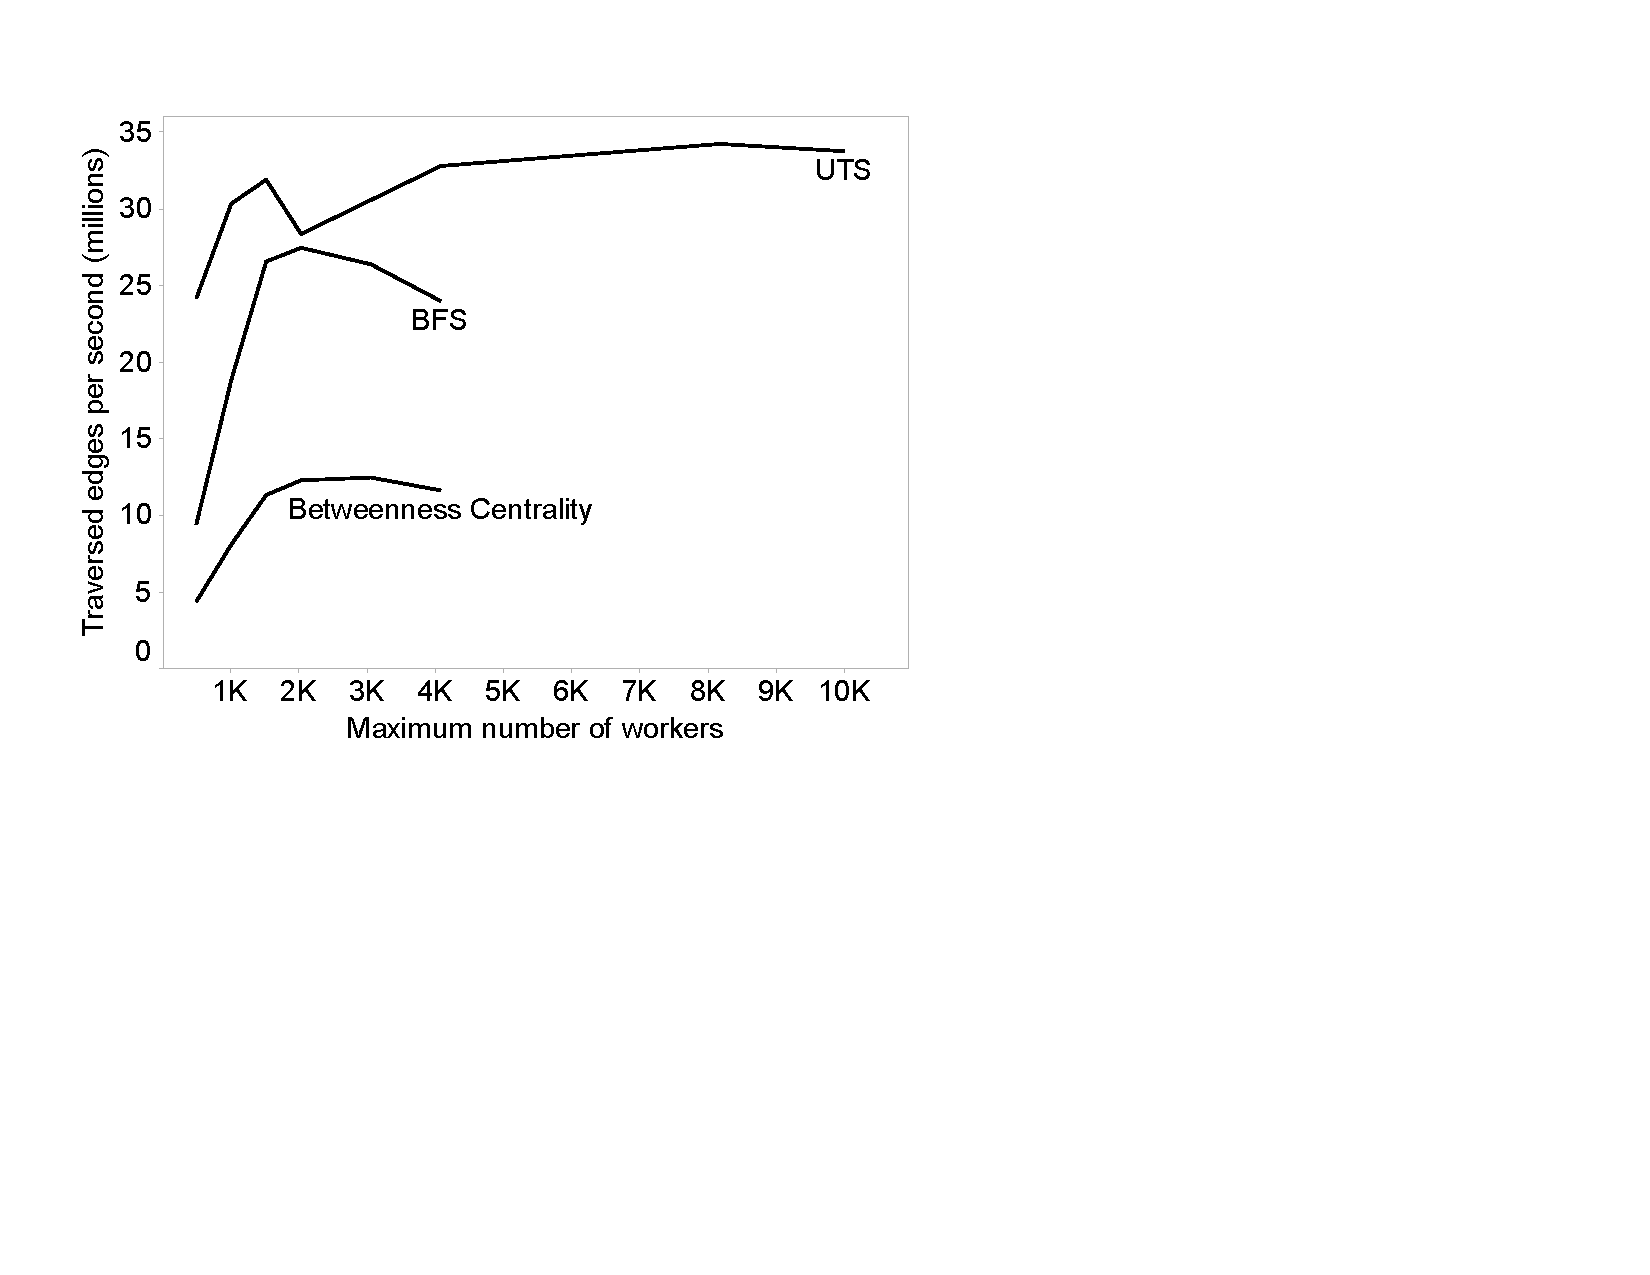
\includegraphics[width=0.95\columnwidth]{figs/worker_sweep}
\begin{minipage}{0.95\columnwidth} 
  \caption{\label{fig:bfs-sweep-workers} Sensitivity to maximum active tasks}
\end{minipage}
\vspace{-3ex}
\end{center}
\end{figure}

\subsubsection{Number of active tasks} \TODO{possibly eliminate}

When a task issues a request that requires a response, it blocks to
allow other tasks to utilize its core. These tasks may also block. To
support the many milliseconds of latency aggregation adds, we need to
support many thousands of blocked tasks. One of the key parameters of
the runtime is the number of blocked tasks allowed; we need enough to
cover the network and aggregation latency, but too many running tasks
can add extra latency as they all must be multiplexed onto the same core.

Figure~\ref{fig:bfs-sweep-workers} shows a sweep of the maximum number
of active tasks (workers) per core for each of our three benchmarks on
16 nodes. The aggregator timeout is set at 1 ms for UTS and 2 ms for
BFS and Betweenness Centrality. The performance peak shifts in this
case, with UTS peaking at 1536 workers, BFS peaking at 2048 workers,
and Betweenness Centrality peaking at 3072 workers. This is the point
where we have enough workers to cover the latency of aggreation. The
different values reflect the different amounts of work done by a task
in each benchmark; UTS does the least, while Betweenness Centrality does the most.

%\subsubsection{Work stealing parameters}
%
%\paragraph{Chunk size}
%
%It is important to steal multiple tasks at a time to both amortize the
%cost of stealing over the network and to spread out work quickly in a
%large system. Figure~\ref{fig:ut_chunksize} shows performance and
%stealing statistics for UTS on \checkme{30} nodes as we increase the stealing chunk size. Recall
%that a thief will take a number of tasks equal to the minimum of half
%the available work or the chunk size; steals fail only when the victim
%has fewer than 2 available tasks. As the scheduler is allowed to
%steal more work beyond 1 task, we see that performance increases up to 6x. This
%shows that the heuristic of stealing the oldest task from victims is
%insufficient alone when a tree-structured computation is imbalanced,
%as observed in \cite{UTS}. By observing sampled state in the execution
%trace, we find that a chunk size as low as 1 allows stealing to
%spread the load evenly across the cluster but cores spend much time
%underutilized as multiple workers wait for steal replies that
%utlimately return little new work.
%
%Performance plateaus before maximum steal amount is limited by the
%size of the victim's task queue. This indicates that artificially limiting steals
%to \checkme{128} tasks does not limit performance. Although a lower
%chunk size limits how quickly work spreads, for sufficient chunk size,
%the heuristic of stealing the oldest tasks from victims in tree-based computations allows for
%stolen work to expand quickly.


%% UTS: chunk size
%\begin{figure}[ht]
%    \begin{center}
%      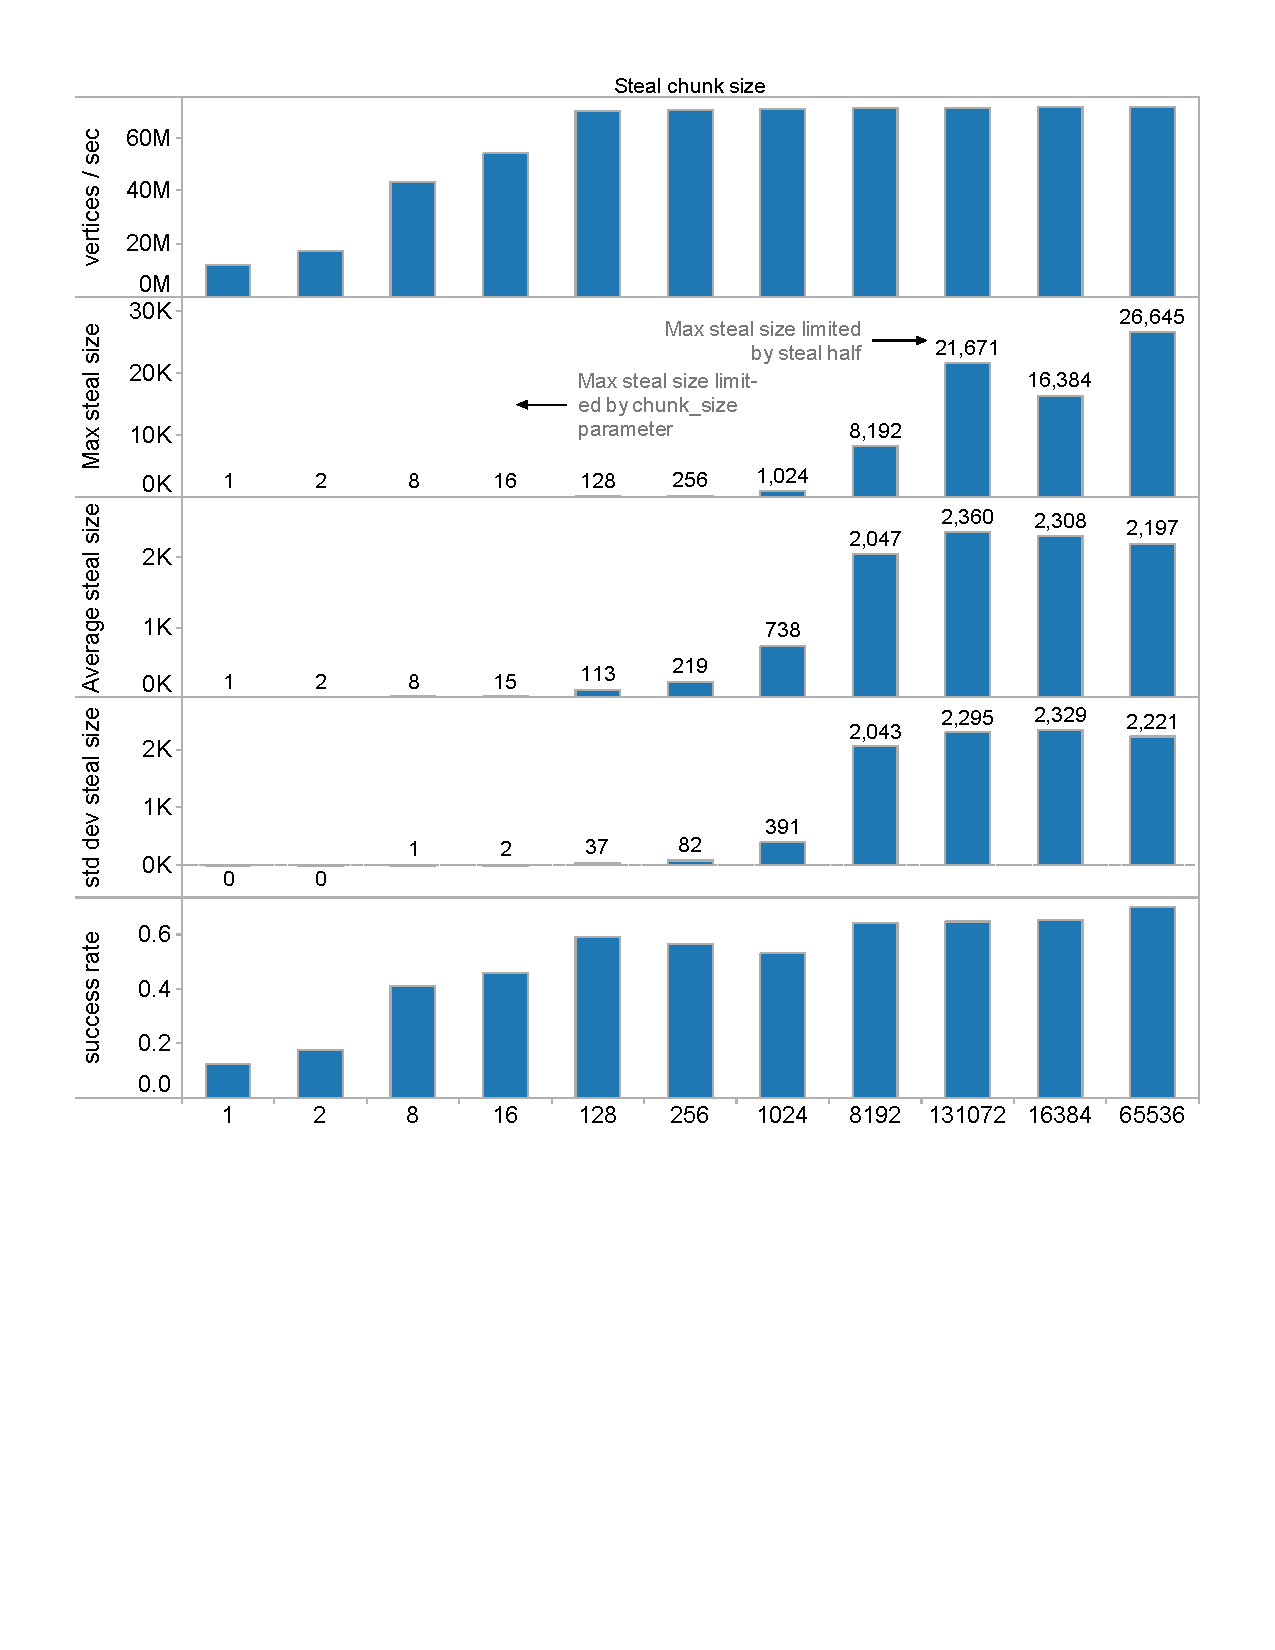
\includegraphics[width=0.5\textwidth]{figs/uts_chunksize.pdf}
%    \end{center}
%    \caption{Performance of UTS-Mem with varying maximum chunk size of
%    steals, run with 30 nodes, 6 cores per node, 4000 workers,
%    \checkme{6M flush ticks}}
%    \label{fig:uts_chunksize}
%\end{figure}


%\TODO{(difference with BFS)}



\subsubsection{Parallel loop threshold}

%\begin{figure}[htb]
%\begin{center}
%  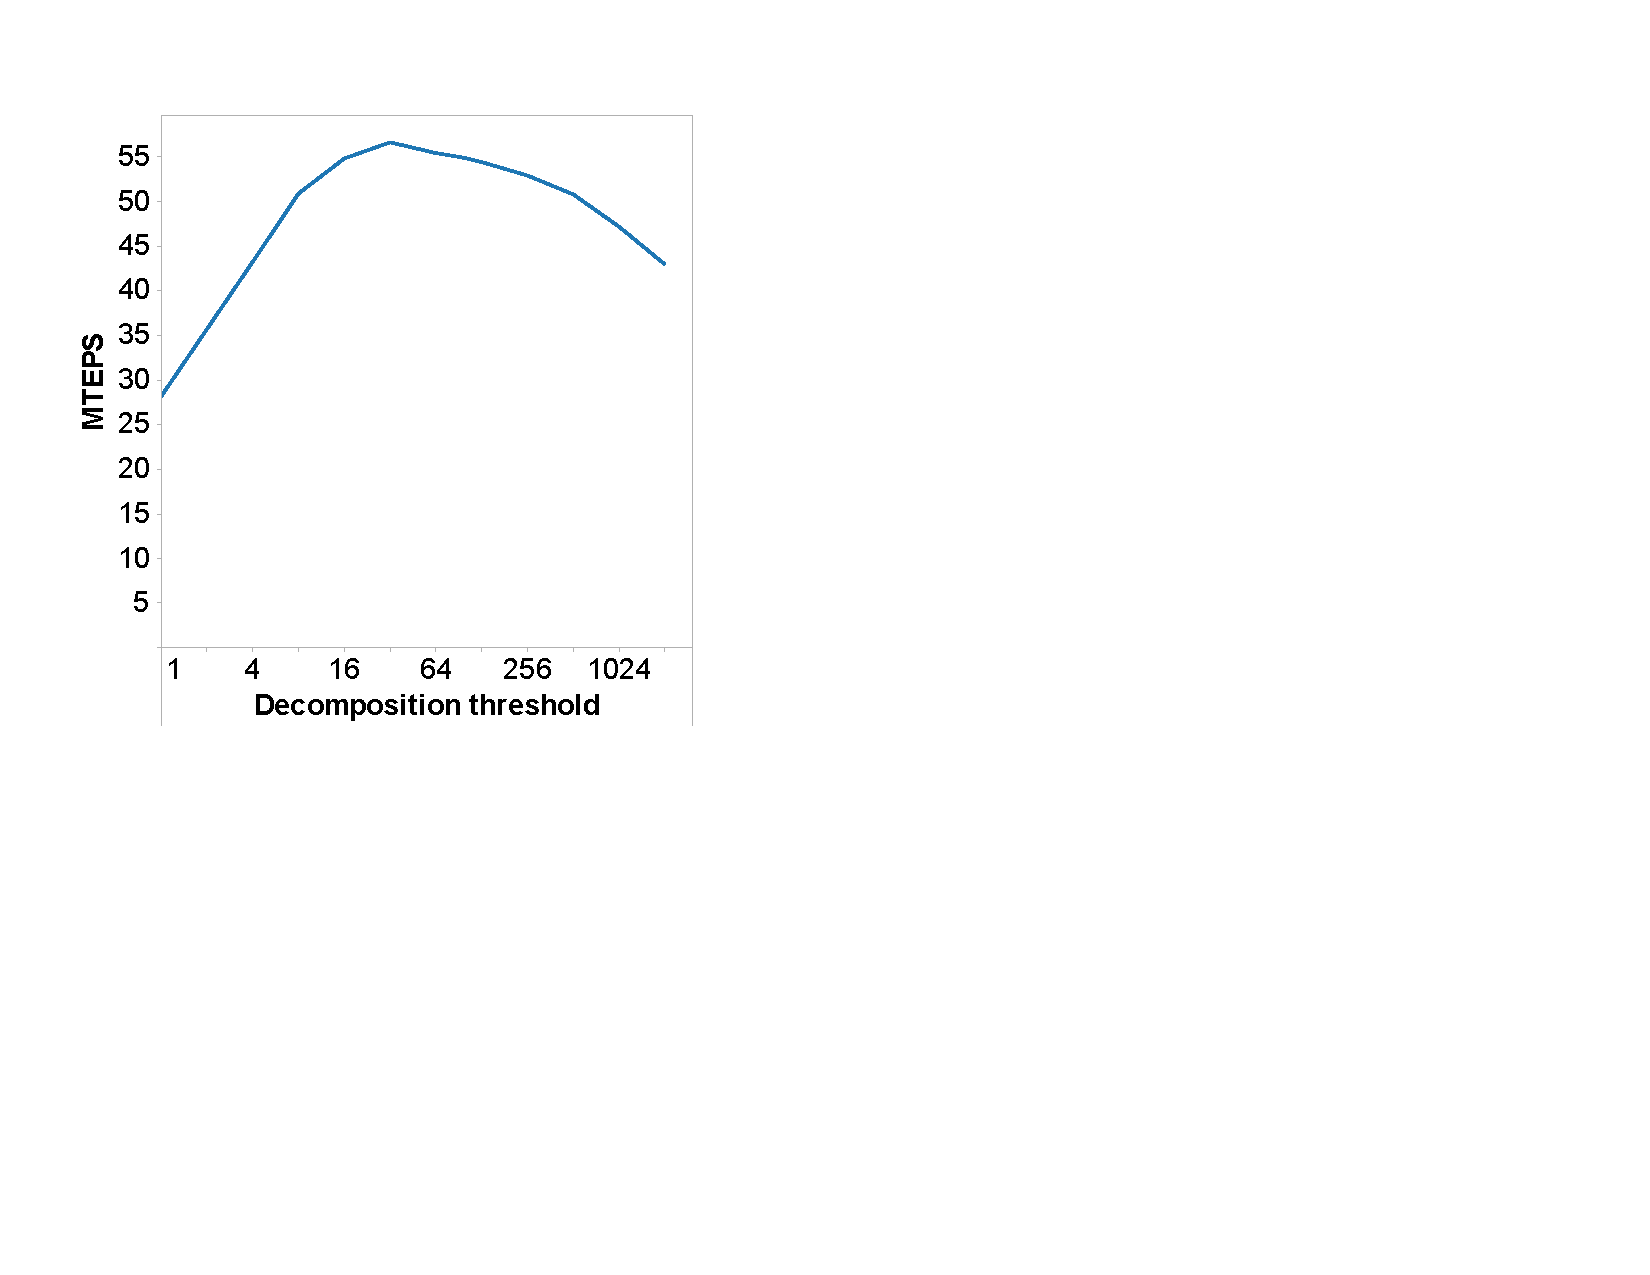
\includegraphics[width=0.95\columnwidth]{figs/bfs_sweep_threshold}
%\begin{minipage}{0.95\columnwidth}
%  \caption{\label{fig:bfs-sweep-threshold} Sensitivity to parallel loop threshold. Note the log scale.}
%\end{minipage}
%\vspace{-3ex}
%\end{center}
%\end{figure}

Parallel overhead---in the form of context switches, task spawns, and
synchronization---can reduce the performance benefit of parallelism.
\Grappa sees a benefit to limiting the amount of parallelism created by
a recursive loop decomposition. The parallel loop threshold (``parallel
granularity'') parameter tells the runtime when to stop creating new tasks and just execute iterations
sequentially. This allows us to amortize the overhead of task
creation. In addition, assigning sequential iterations to a single
task provides the potential to exploit locality when data for adjacent iterations is
also adjacent in memory. The ability to exploit this locality that
exists in the application is an important advantage. We found that in UTS and BFS, increasing the
threshold from 1 up to 8 or 16, respectively, increases performance by
more than 60\%.


% uts threshold
%\begin{figure}[ht]
%    \begin{center}
%      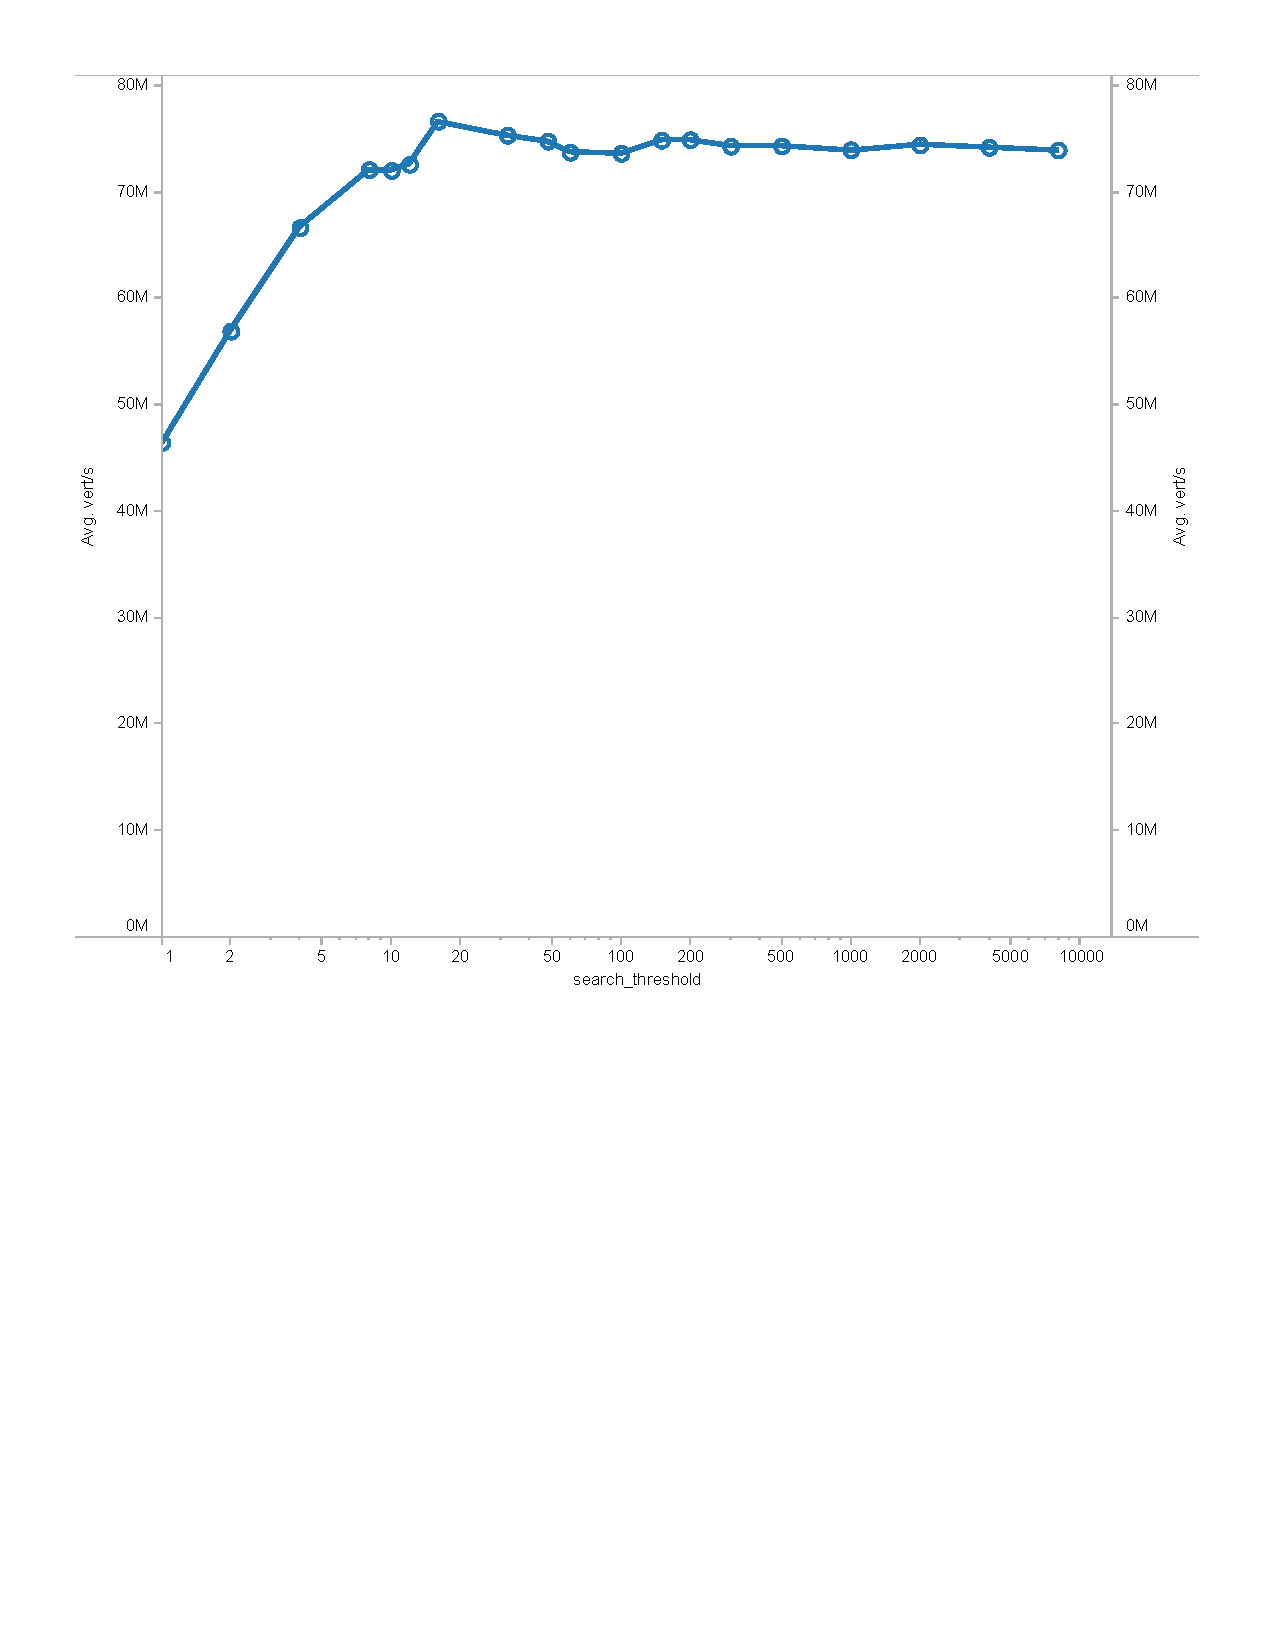
\includegraphics[width=0.5\textwidth]{figs/uts_threshold.pdf}
%    \end{center}
%    \caption{Performance of UTS-Mem with varying parallel loop
%        threshold, run with 30 nodes, 6 cores per node, 4000 workers,
%    \checkme{6M flush ticks}}
%    \label{fig:uts_threshold}
%\end{figure}

\subsection{Summary}\TODO{this is a placeholder: do we need this section?}

\paragraph{Context-switch overhead.} Should we also compare with other packages? (Maybe Capriccio, QThreads?, or even real OS threads?)

\paragraph{Latency.} Measure remote data access latency with and without aggregation turned on.

\paragraph{Aggregated message sizes.} Characterization of the resulting message sizes with aggregation. Right now we only have message size vs. bandwidth.

\paragraph{Utilization.} CPU utilization, Memory, Network. It would be great to answer the question of where is our bottleneck right now. Amount of concurrency with and without aggregation. 

\paragraph{Memory accesses.} Rate of accesses to remote data. Rate of delegate ops. Show limit with GUPs.



%Retries are performed by the memory controller when remote synchronization operations fail to find the full-bit associated with each memory location in the unavailable state.  Retries are issued at low priority relative to new memory operations issued by the processor by other contexts, so they consume what would otherwise be unused injection bandwidth.  On a full-bandwidth system such as the MTA-2, retries have no impact on the progress of tasks other than their own.  On a Cray XMT, network bandwidth is limited, so retries create congestion.  In comparison, \Grappa performs synchronization without retries, delaying responses at the receiving end until ready to notify the sender to proceed.  This saves bandwidth and permits scaling of tasks performing synchronization even on low injection rate networks.


%\begin{figure*}[ht]
%    \begin{minipage}{0.3\linewidth}
%        \centering
%        \includegraphics[width=\textwidth]{figs/chunksize-uts.pdf}
%        \caption{chunksize caption}
%        \label{fig:chunksize-uts}
%    \end{minipage}
%    \begin{minipage}{0.3\linewidth}
%        \centering
%        \includegraphics[width=\textwidth]{figs/workers-uts.pdf}
%        \caption{workers caption}
%        \label{fig:workers-uts}
%    \end{minipage}
%    \begin{minipage}{0.3\linewidth}
%        \centering
%        \includegraphics[width=\textwidth]{figs/thresh-uts.pdf}
%        \caption{threshold caption}
%        \label{fig:thresh-uts}
%    \end{minipage}
%\end{figure*}

}

\section{Related work}

Ways to organize this:
Approaches to graphs: special purpose XMT -> cluster -> distributed frameworks {pregel,graphlab} -> limited programming model -> grappa gen purpose



\subsection{Multithreading to tolerate latency}
Using multithreading to tolerate memory latency is well-covered in the literature. Hardware implementations include the Tera MTA \cite{Tera}, Cray XMT \cite{}, Simultaneous multithreading \cite{}, MIT Alewife \cite{}, Cyclops \cite{}, and even GPUs \cite{fatahalian}.

software threads
lightweight threading

RAMCloud takes a different approach and argues for optimizing networked systems for very low latency with the motivation of getting good performance regardless of access pattern, as well as reducing latency of recovery to reduce backup storage costs.


\subsection{Distribute Shared Memory}

Grappa includes a software distributed shared memory (SDSM). Many traditional SDSM systems are page based [Treadmarks,...], and a lot of work deals with maintaining consistency of data efficiently and optimizing for sharing. Grappa's shared memory is implemented by Active Messages and there is no caching under the hood. Every piece of memory in the shared address space belongs to a single core, and data can be accessed incoherently at any granularity. Grappa provides an API for explicit incoherent caching to take advantage of locality where it exists, as well as sharing. 

Shared memory systems often try to reduce the cost of memory access by predicting good prefetches to overlap memory access and computation; however, this is less effective for irregular applications with fine-grained, data-dependent memory accesses. Grappa depends on high amounts of concurrency to tolerate latency with multithreading.

SDSM systems are usually built to be programmed with flat shared memory programming models like OpenMP, rather than models that make locality explicit like PGAS. 


GASNet is a networking library for supporting portable implmentations of global address space applications or languages, like UPC and recently Chapel...
Grappa currently uses GASNet for networking, but does not use gasnet's mapped shared memory segments for supporting RDMA. Rather, the global address space is implemented at a higher level using Active Messages.

RAMCloud - RPC call communication abstraction like us because it supports more flexibility,...


Difference from txDSM \cite{sdsm-with-txn-coherence} is that we don't try to provide txns over multiple nodes, only within one core's memory.

\subsection{Partitioned Global Address space}
The goal of presenting a global view of distributed memory to the programmer is shared by the PGAS community, and is used in languages like Chapel \cite{Chapel}, X10 \cite{X10}, and UPC \cite{UPC}. In these programming models, access to shared structures look like normal memory references, but the programmer tries to minimize references to remote nodes. Unlike the usual programming goal in PGAS, since we target problems with poor locality, we design Grappa for remote references as a common case. Thread private data is still local, and unlike the XMT, we exploit locality where it does exist in an application (such as spatial locality in a graph edgelist), but we design the system to perform well in the midst of mostly remote accesses to large shared data structures. We would like to implement PGAS languages that support dynamic parallelism, like Chapel, in Grappa.

\subsection{Programming models for distributed graph processing}

Distributed graph processing frameworks like Pregel \cite{pregel:2010} and Distributed GraphLab \cite{distgraphlab:vldb12} provide graph-parallel, vertex-centric programming abstractions that free the application writer from solving distributed system issues like scheduling parallelism, handling fault tolerance, and scaling communication. Pregel adopts a bulk-synchronous parallel (BSP) execution model, which makes it inefficient on workloads that could prioritize vertices. GraphLab, on the other hand, schedules vertex computations individually, allowing prioritization, which gives faster convergence in a variety of iterative algorithms. Grappa also supports dynamic parallelism with asynchronous execution, but has a more general purpose programming model, where parallelism is expressed as tasks or loop iterations. \TODO{and express locality? How much to talk about how graphlab achieves scalable performance?}

\TODO{should we mention GreenMarl and how its first distributed try is compile down to Pregel}

\section{Conclusion}
In PGAS implementations there is typically a large discrepancy between the first, simple, description of an algorithm and the final, optimized one. At the core of this work is the desire to have a library of data structures which can be used without worrying about when they will be consistent or whether they will limit scalability.
Bringing findings from shared memory into the PGAS domain brings with it new challenges and opportunities.
We have shown that the additional concurrency that comes with a latency-tolerant runtime, rather than compounding the problem, provides a new opportunity for reducing communication by combining locally.
% perform some of the locality optimizations that finely-tuned implementations would.
This allows flat-combined sequentially-consistent global data structures to scale well out to a thousand cores with millions of concurrent threads.


\bibliographystyle{abbrv}
\bibliography{paper}

\end{document}

